\chapter{Analysis}

\section{Introduction}
Following the initial feasibility study conducted in Chapter 2, this chapter presents a comprehensive analysis of Alpha Net's Network Department operations. The analysis phase is crucial for understanding the current state of the organization, identifying key challenges, and establishing a foundation for proposed solutions. This chapter employs multiple analytical approaches including literature review, procedural analysis, form evaluation, and on-site observations to provide a holistic view of the organization's operational dynamics.

The analysis encompasses both theoretical frameworks derived from existing literature and practical observations gathered through direct engagement with Alpha Net's operations. By combining these approaches, we aim to develop a thorough understanding of the organizational challenges and opportunities that will inform the subsequent design and implementation phases of this project.

This analytical framework addresses the key problems identified in the feasibility study, including technical awareness gaps among SME clients, internal communication inefficiencies, limited automation in customer support, and infrastructure dependencies. The findings presented in this chapter will serve as the empirical foundation for developing targeted solutions that enhance operational efficiency and service delivery quality.

\section{Information Gathering}

The information gathering phase employed a multi-faceted approach to ensure comprehensive data collection and analysis. As illustrated in Figure \ref{fig:info_gathering_components}, the information gathering process was systematically divided into four distinct components, each contributing unique insights to the overall analysis.

\begin{figure}[H]
    \centering
    \begin{tikzpicture}[
        node distance=2cm,
        every node/.style={align=center, font=\footnotesize},
        box/.style={rectangle, draw, fill=blue!10, minimum width=3cm, minimum height=1.5cm, rounded corners=3pt},
        main/.style={rectangle, draw, fill=green!20, minimum width=4cm, minimum height=1cm, rounded corners=5pt, font=\small\bfseries}
    ]
        % Main node
        \node[main] (main) {Information Gathering};
        
        % Four components
        \node[box, below left=1.5cm and 2cm of main] (literature) {3.2.1\\Review of Literature,\\Procedure and Forms};
        \node[box, below right=1.5cm and 2cm of main] (observation) {3.2.2\\On Site\\Observation};
        \node[box, below left=3cm and 2cm of main] (interviews) {3.2.3\\Interviews};
        \node[box, below right=3cm and 2cm of main] (questionnaires) {3.2.4\\Questionnaires};
        
        % Arrows
        \draw[->, thick] (main) -- (literature);
        \draw[->, thick] (main) -- (observation);
        \draw[->, thick] (main) -- (interviews);
        \draw[->, thick] (main) -- (questionnaires);
    \end{tikzpicture}
    \caption{Components of Information Gathering Process}
    \label{fig:info_gathering_components}
\end{figure}

This comprehensive approach ensures that data is collected from multiple sources and perspectives, providing a robust foundation for analysis and subsequent recommendations.

\subsection{Review of Literature, Procedure and Forms}
The literature review and procedural analysis phase involved a comprehensive examination of existing documentation, operational procedures, and standardized forms used within Alpha Net's Network Department. This systematic review provided insights into the theoretical foundations underlying current practices and identified gaps between established best practices and current implementation.

\subsubsection*{Literature Review Methodology}
The literature review was conducted through comprehensive analysis of Alpha Net's digital presence, service documentation, and industry positioning. The review encompassed several key areas derived from the company's website analysis:

\begin{itemize}
    \item Enterprise-level cloud and technology solutions architecture, focusing on Alpha Net's 24+ years of experience in IT infrastructure
    \item Multi-data center hosting strategies across USA and Bangladesh with emphasis on BDIX connectivity and Gbps networking
\begin{figure}[H]
    \centering
    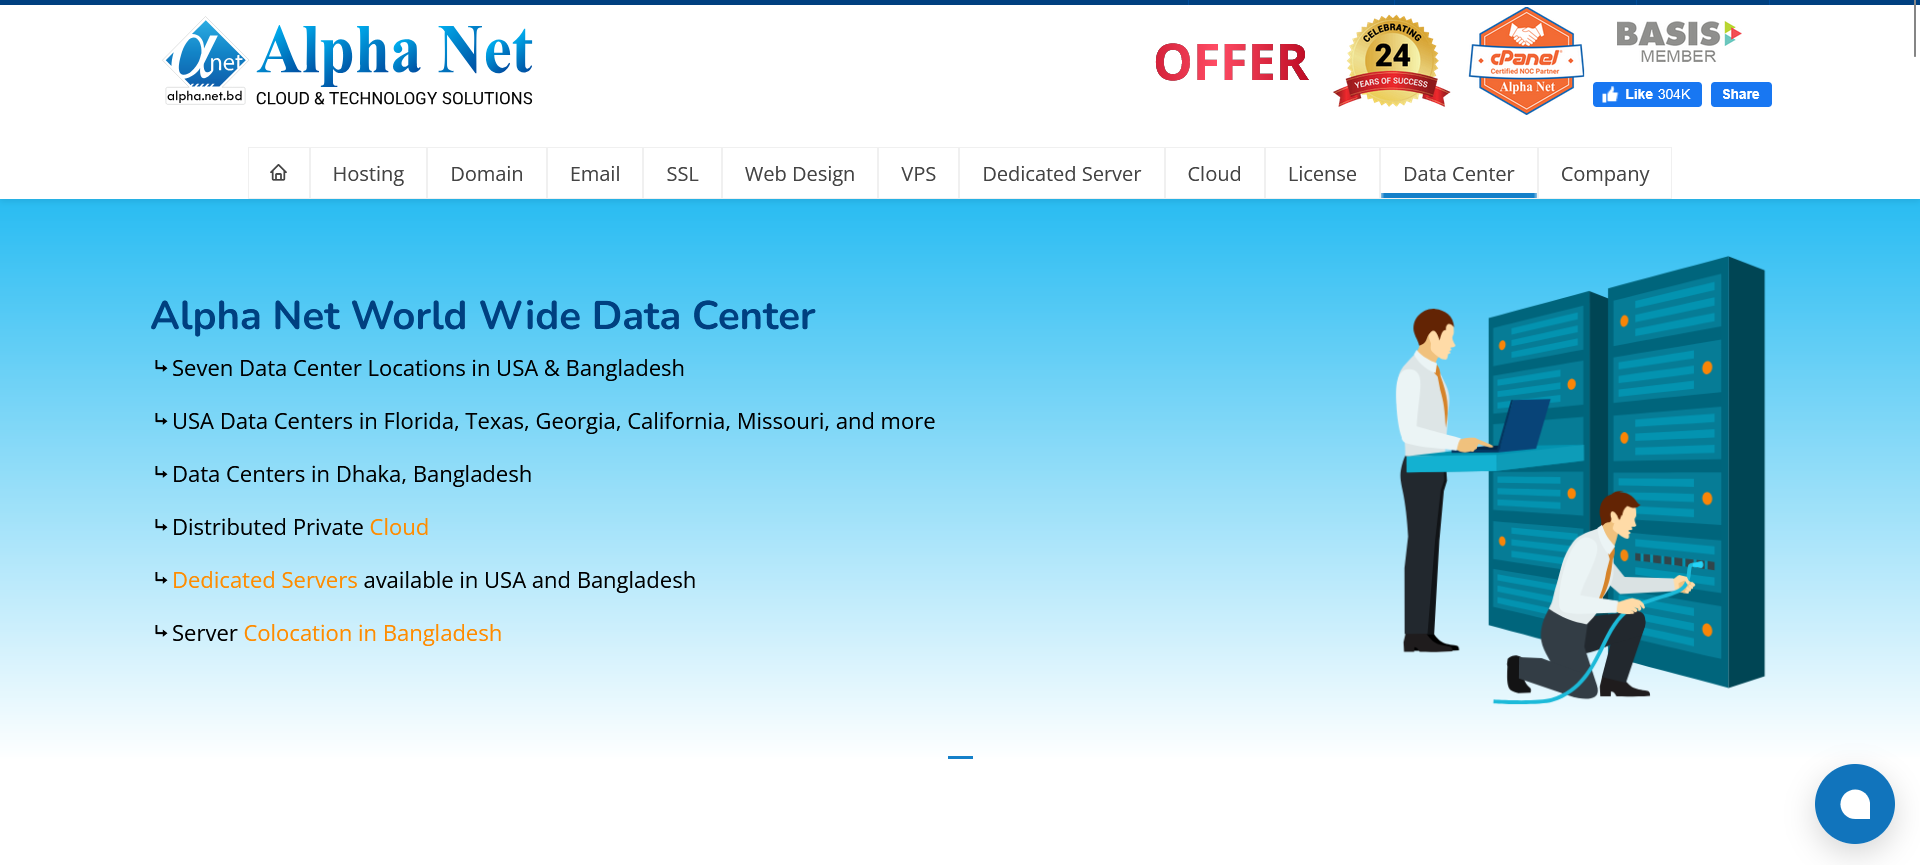
\includegraphics[width=0.8\textwidth]{Photos/datacenter.png}
    \caption{Alpha Net's Data Center Infrastructure highlighting worldwide connectivity and enterprise-level hosting solutions}
    \label{fig:datacenter}
\end{figure}
    \item Service portfolio analysis including dedicated servers (Xeon Gold \& Platinum Series), VPS hosting, web hosting, business email solutions, and telecommunication services
\begin{figure}[H]
    \centering
    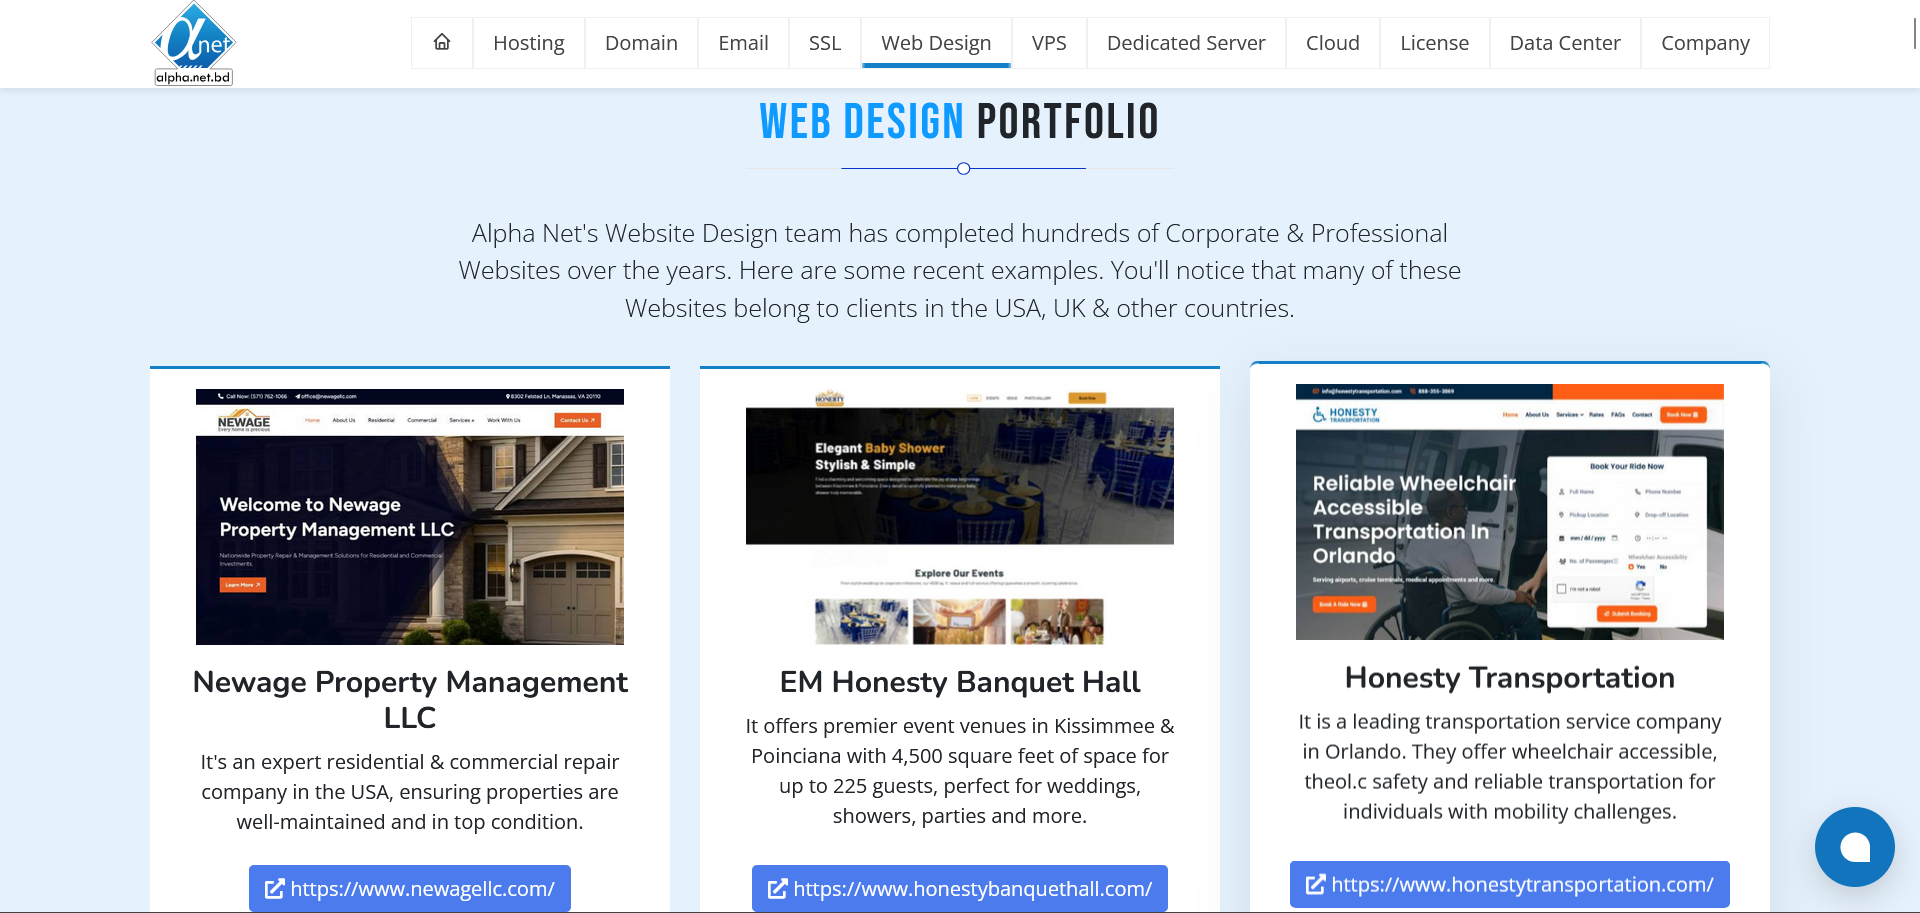
\includegraphics[width=0.9\textwidth]{Photos/portfolio.png}
    \caption{Alpha Net's Web Design Portfolio showcasing corporate and professional websites across multiple industries}
    \label{fig:portfolio}
\end{figure}
    \item Technology partnership frameworks with major providers including AWS, Microsoft Azure, Google Cloud, CloudFlare, Oracle, and specialized hosting technologies
    \item Customer relationship management approaches for serving 5000+ customers across 60+ countries
    \item Payment gateway integration and multi-currency support systems for Bangladesh and international markets
\begin{figure}[H]
    \centering
    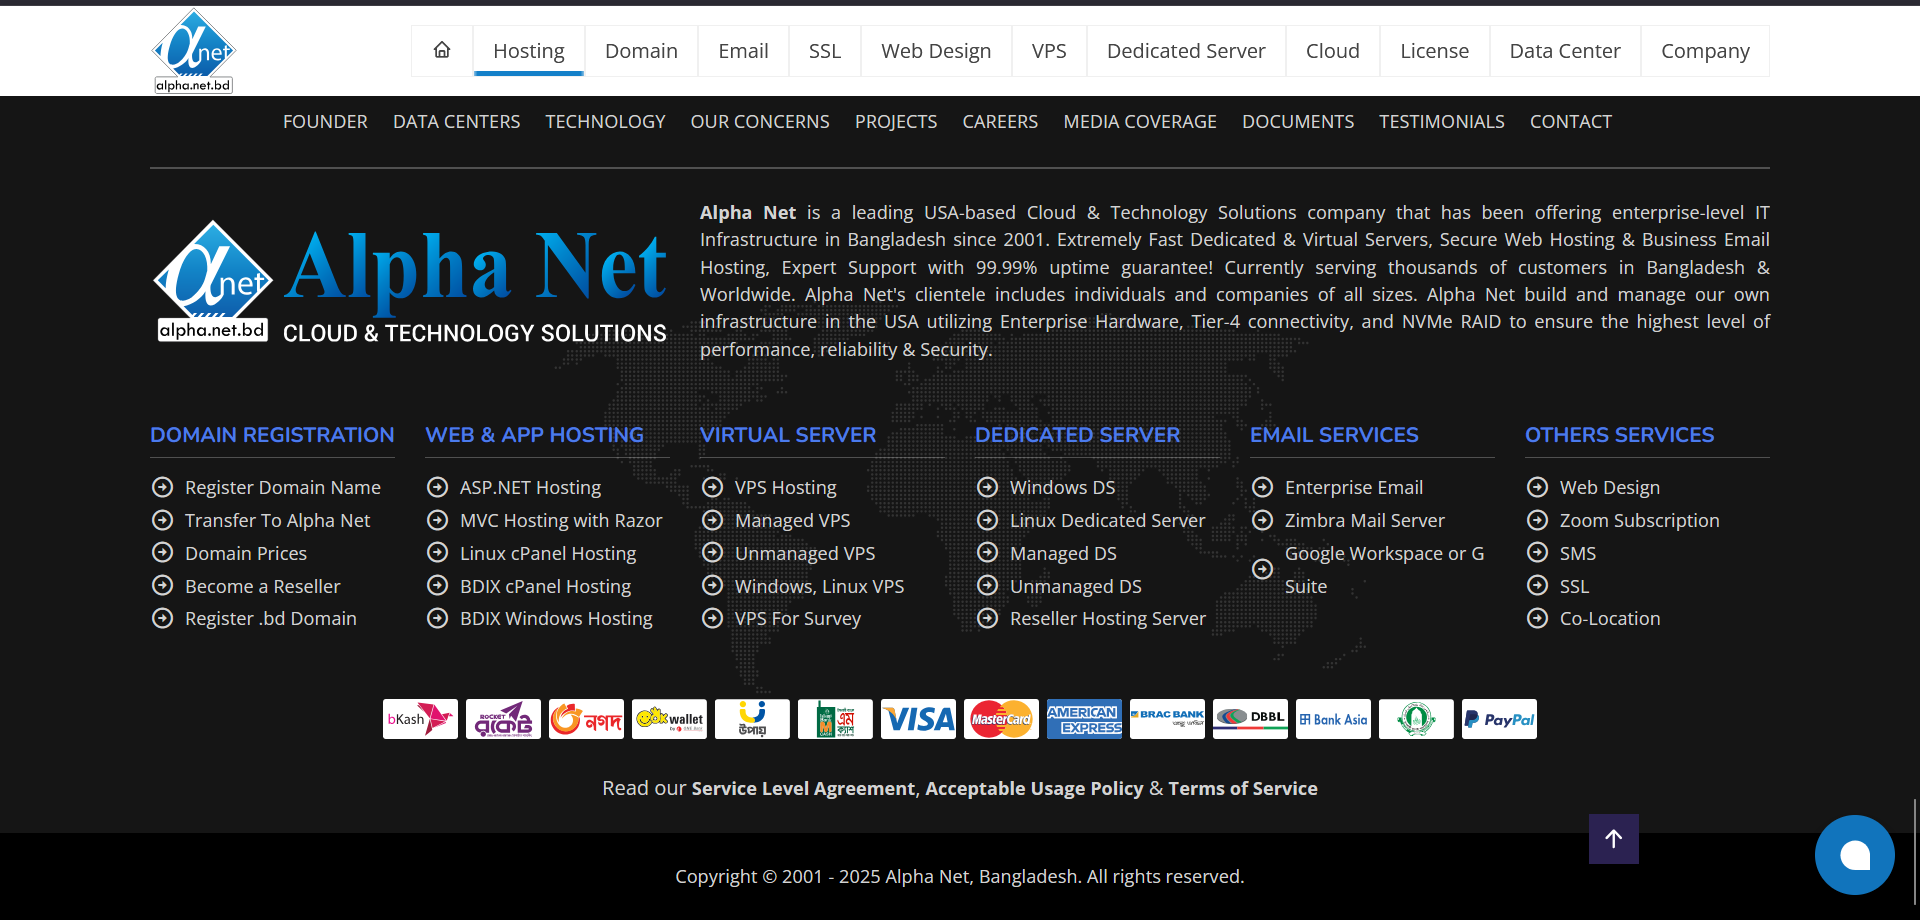
\includegraphics[width=0.8\textwidth]{Photos/payment.png}
    \caption{Alpha Net's Payment Gateway Integration supporting multiple payment methods including mobile banking and international gateways}
    \label{fig:payment}
\end{figure}
\end{itemize}



The literature review revealed that Alpha Net's comprehensive service portfolio positions it as a leading technology solutions provider in Bangladesh. The company's integration of international technology partnerships with local market understanding demonstrates best practices in cross-cultural IT service delivery. However, opportunities exist for enhanced automation in customer onboarding processes and improved self-service capabilities for SME clients.

\subsubsection*{Procedural Analysis}
Alpha Net's operational procedures were systematically analyzed through website functionality examination, service delivery workflows, and customer interaction protocols:

\begin{itemize}
    \item Domain registration and hosting service provisioning through automated portal systems with instant activation capabilities
\begin{figure}[H]
    \centering
    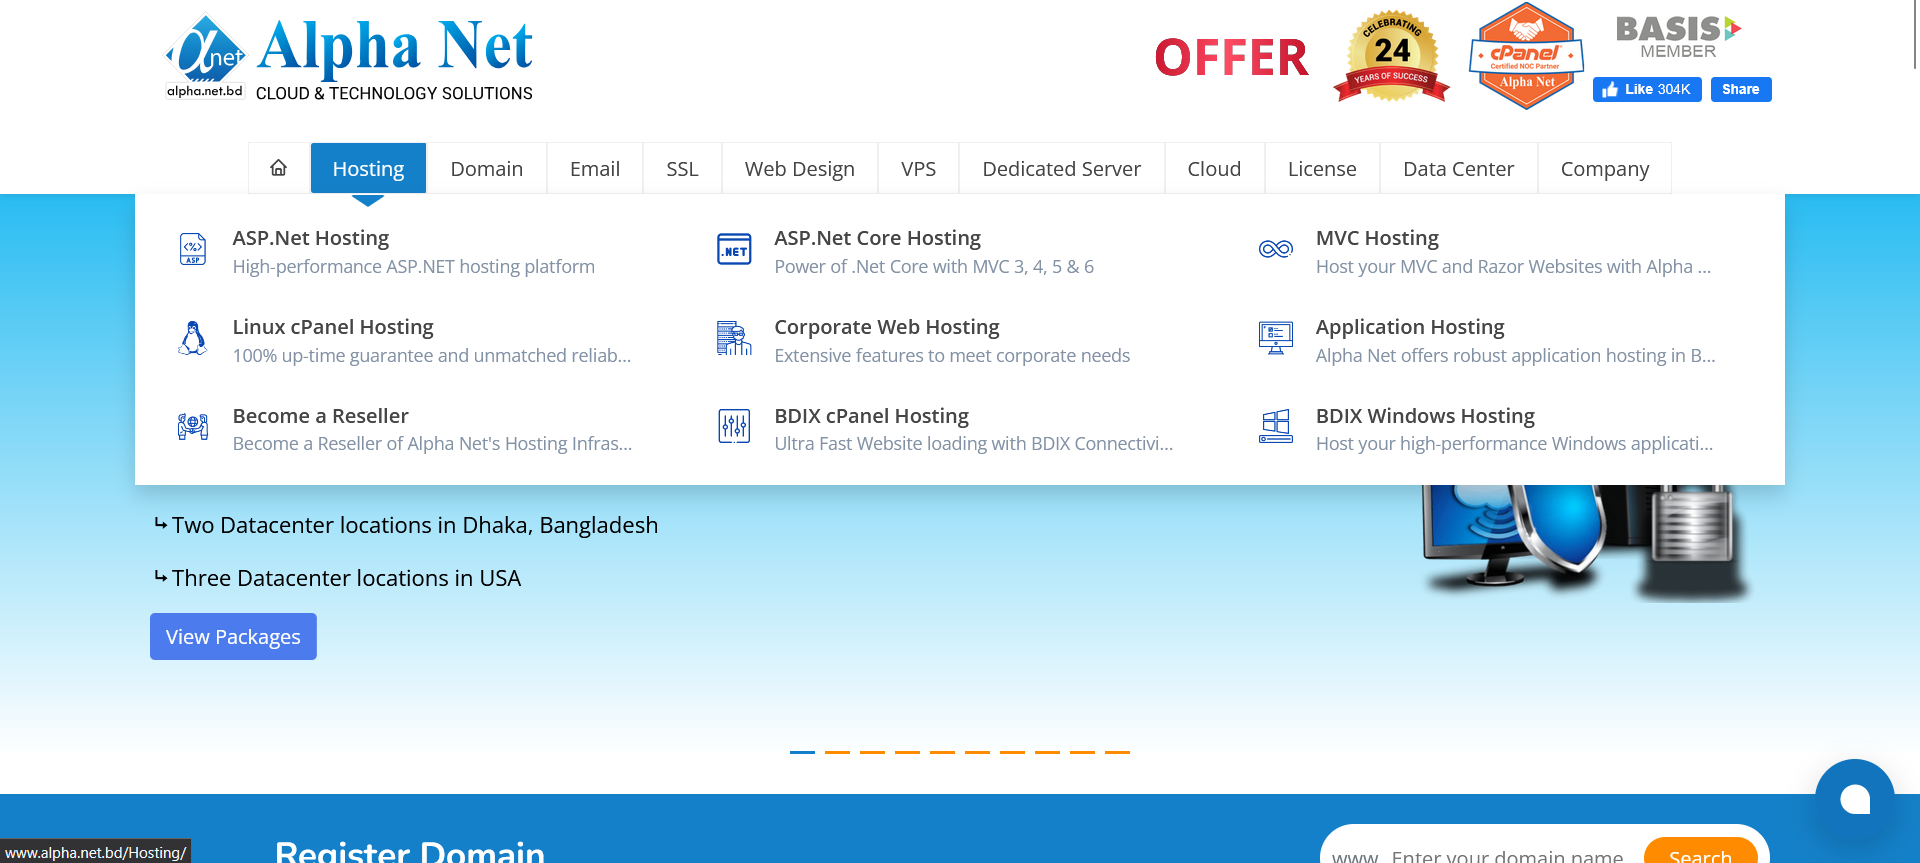
\includegraphics[width=0.8\textwidth]{Photos/hosting.png}
    \caption{Domain name search}
    \label{fig:hosting}
\end{figure}
    \item Multi-tier hosting architecture supporting both shared hosting (Linux cPanel, Windows ASP.NET) and enterprise solutions (dedicated servers, VPS)
    \item Business communication services including Cloud PBX, email hosting (Zimbra, Google Workspace), and SMS marketing platforms
    \item SSL certificate management and website security implementation across multiple certificate authorities
    \begin{figure}[H]
        \centering
        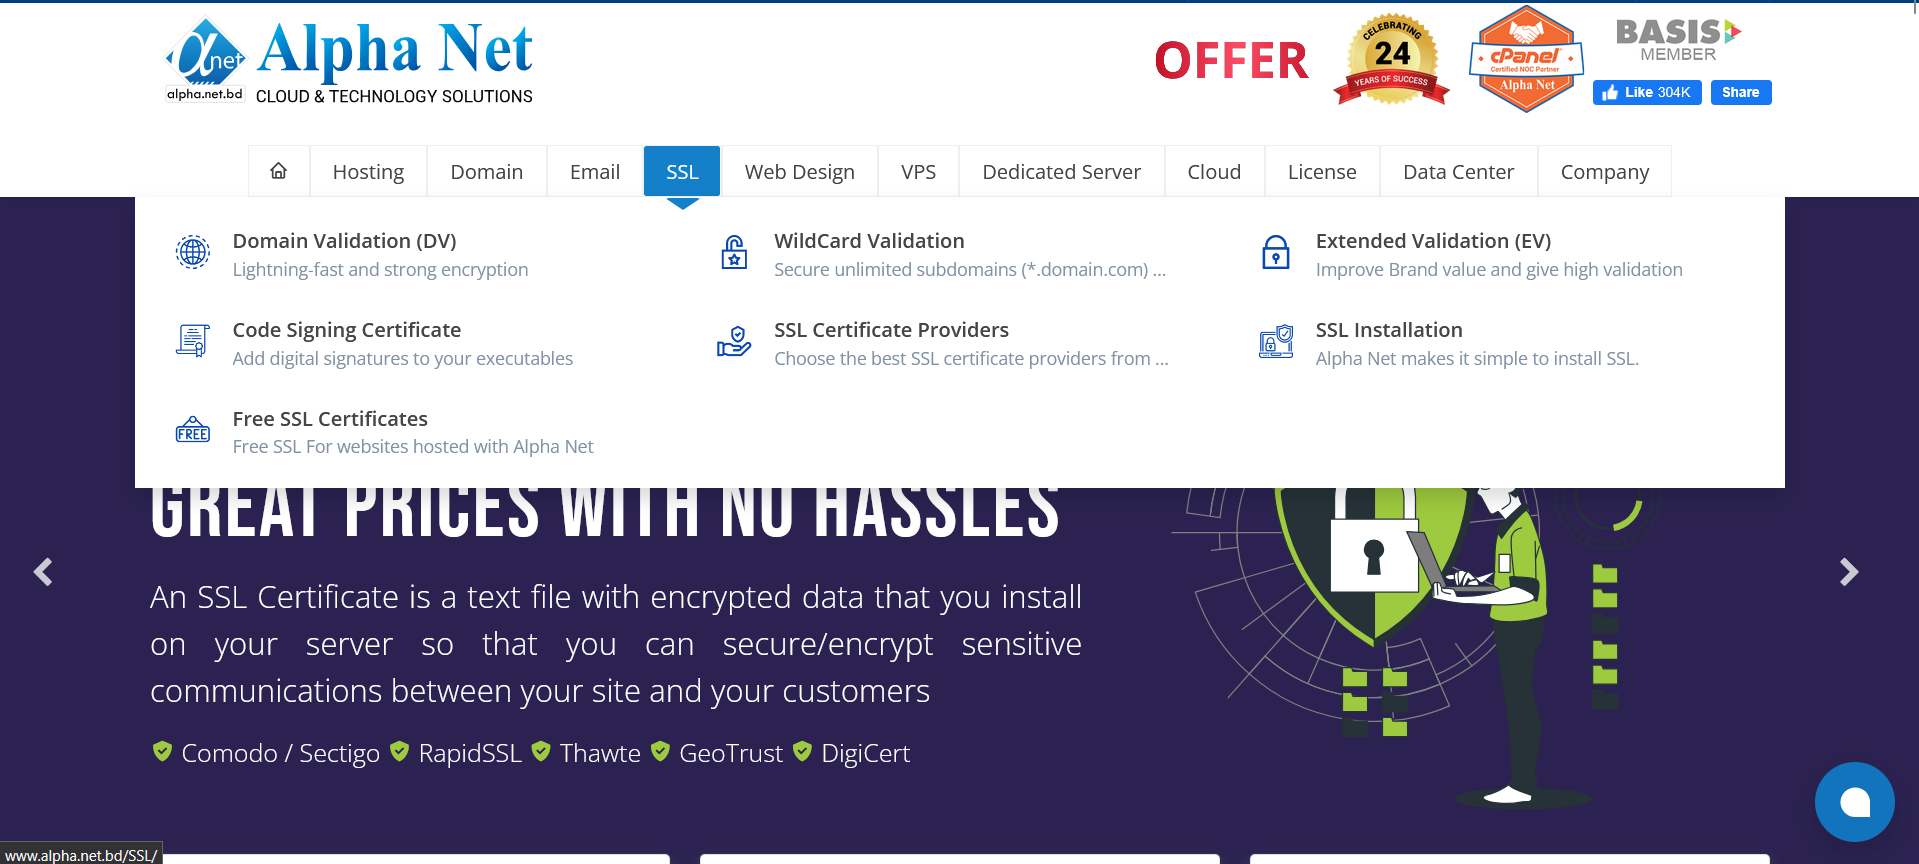
\includegraphics[width=0.9\textwidth]{Photos/ssl.png}
        \caption{SSL Certificate Management and Security Implementation}
        \label{fig:ssl}
    \end{figure}
    \item Technical support delivery through 24/7 live chat, phone support (+880 9613 250 250), and ticketing systems
    \begin{figure}[H]
        \centering
        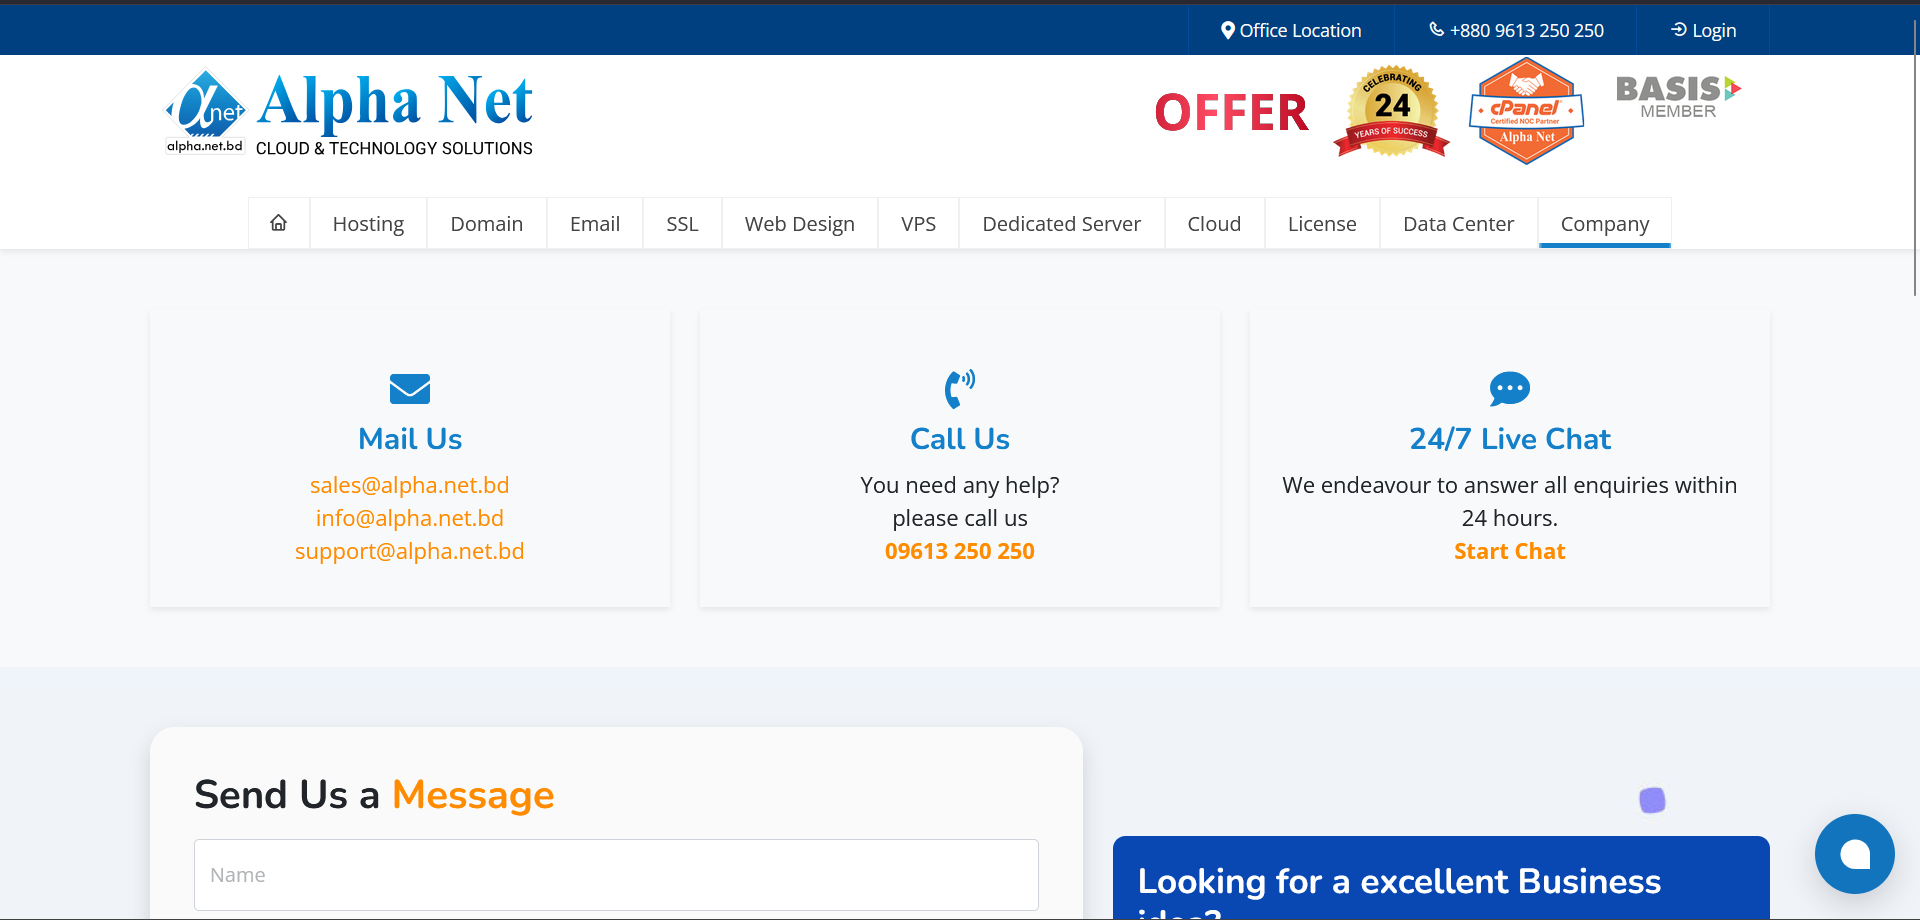
\includegraphics[width=0.9\textwidth]{Photos/chat.png}
        \caption{24/7 Live Chat and Technical Support}
        \label{fig:chat}
    \end{figure}
    \item Payment processing workflows supporting 14+ payment methods including mobile banking (bKash, Rocket, Nagad), traditional banking, and international payment gateways
    % Payment image already used above, but can be referenced if needed
\end{itemize}



The procedural analysis identified Alpha Net's strength in providing integrated technology solutions with robust technical infrastructure. The company's procedures effectively serve both local Bangladeshi clients and international customers. Areas for improvement include streamlining the service selection process for non-technical clients and enhancing automated monitoring capabilities for proactive issue resolution.

\subsubsection*{Form Evaluation}
Digital forms and user interfaces were evaluated through Alpha Net's web portal, client interaction systems, and service request workflows:

\begin{itemize}
    \item Domain search and registration forms with real-time availability checking and instant registration capabilities
    \begin{figure}[H]
        \centering
        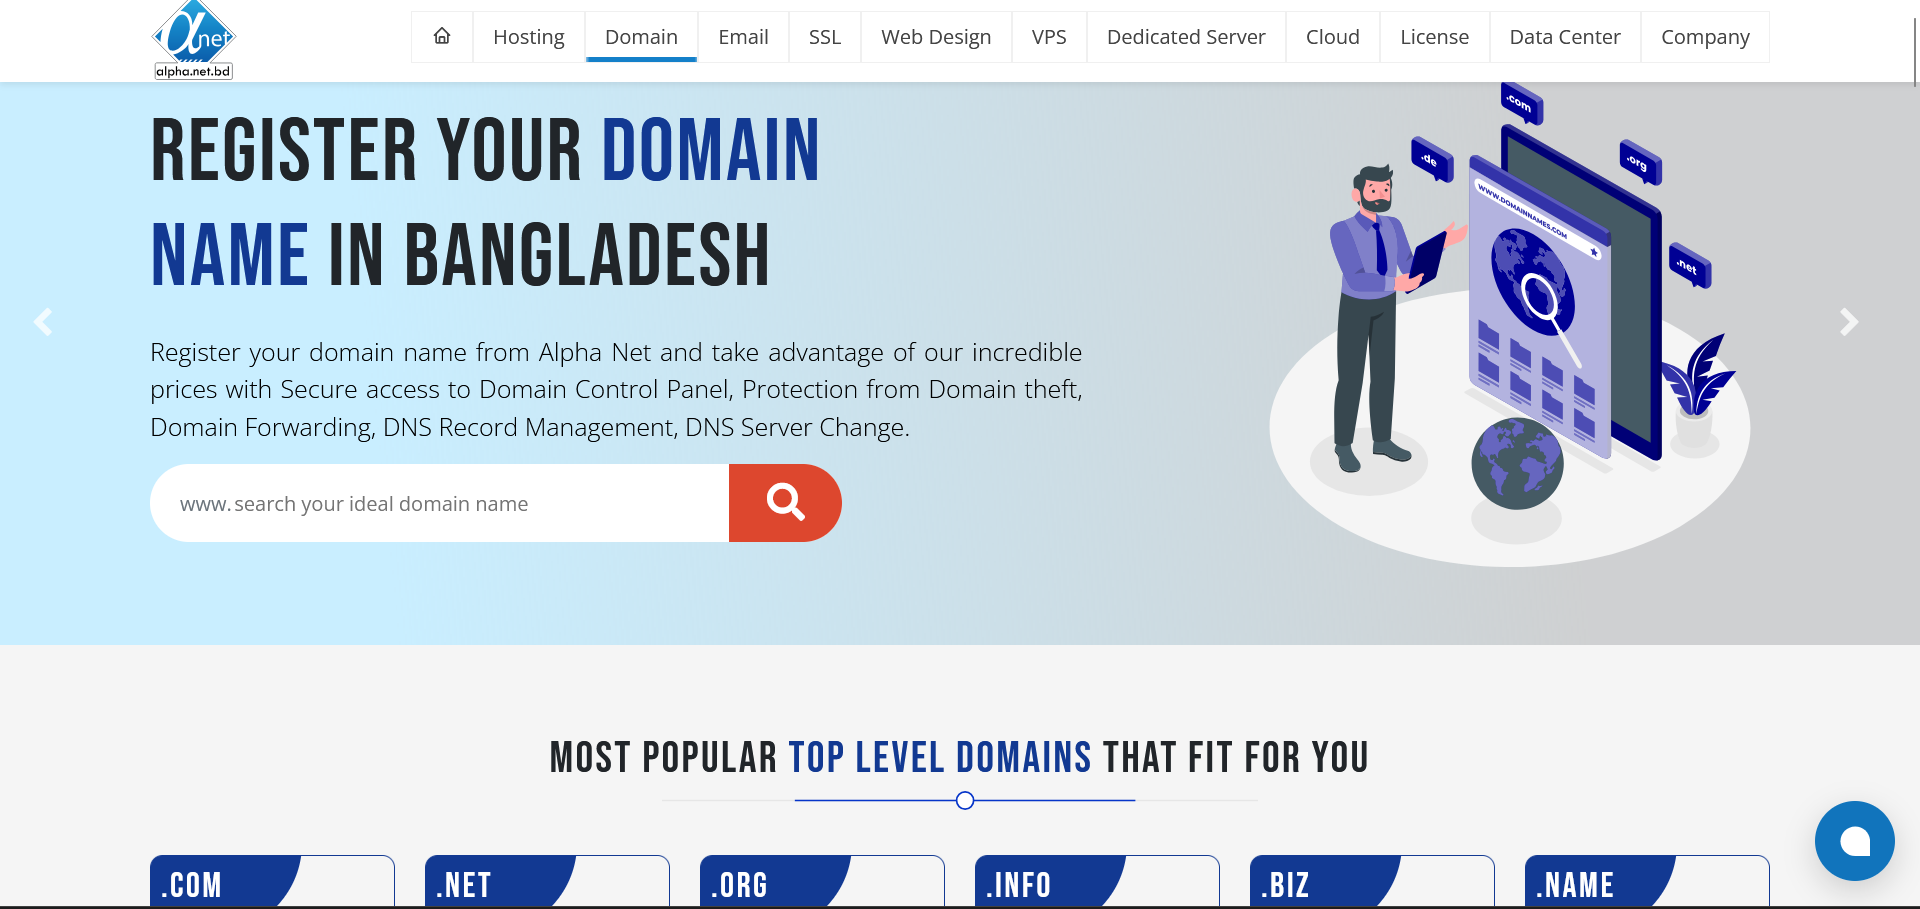
\includegraphics[width=0.9\textwidth]{Photos/domain.png}
        \caption{Domain Name Search}
        \label{fig:domain_registration}
    \end{figure}
    \item Client portal functionality for account management, billing, and support ticket submission
    \begin{figure}[H]
        \centering
        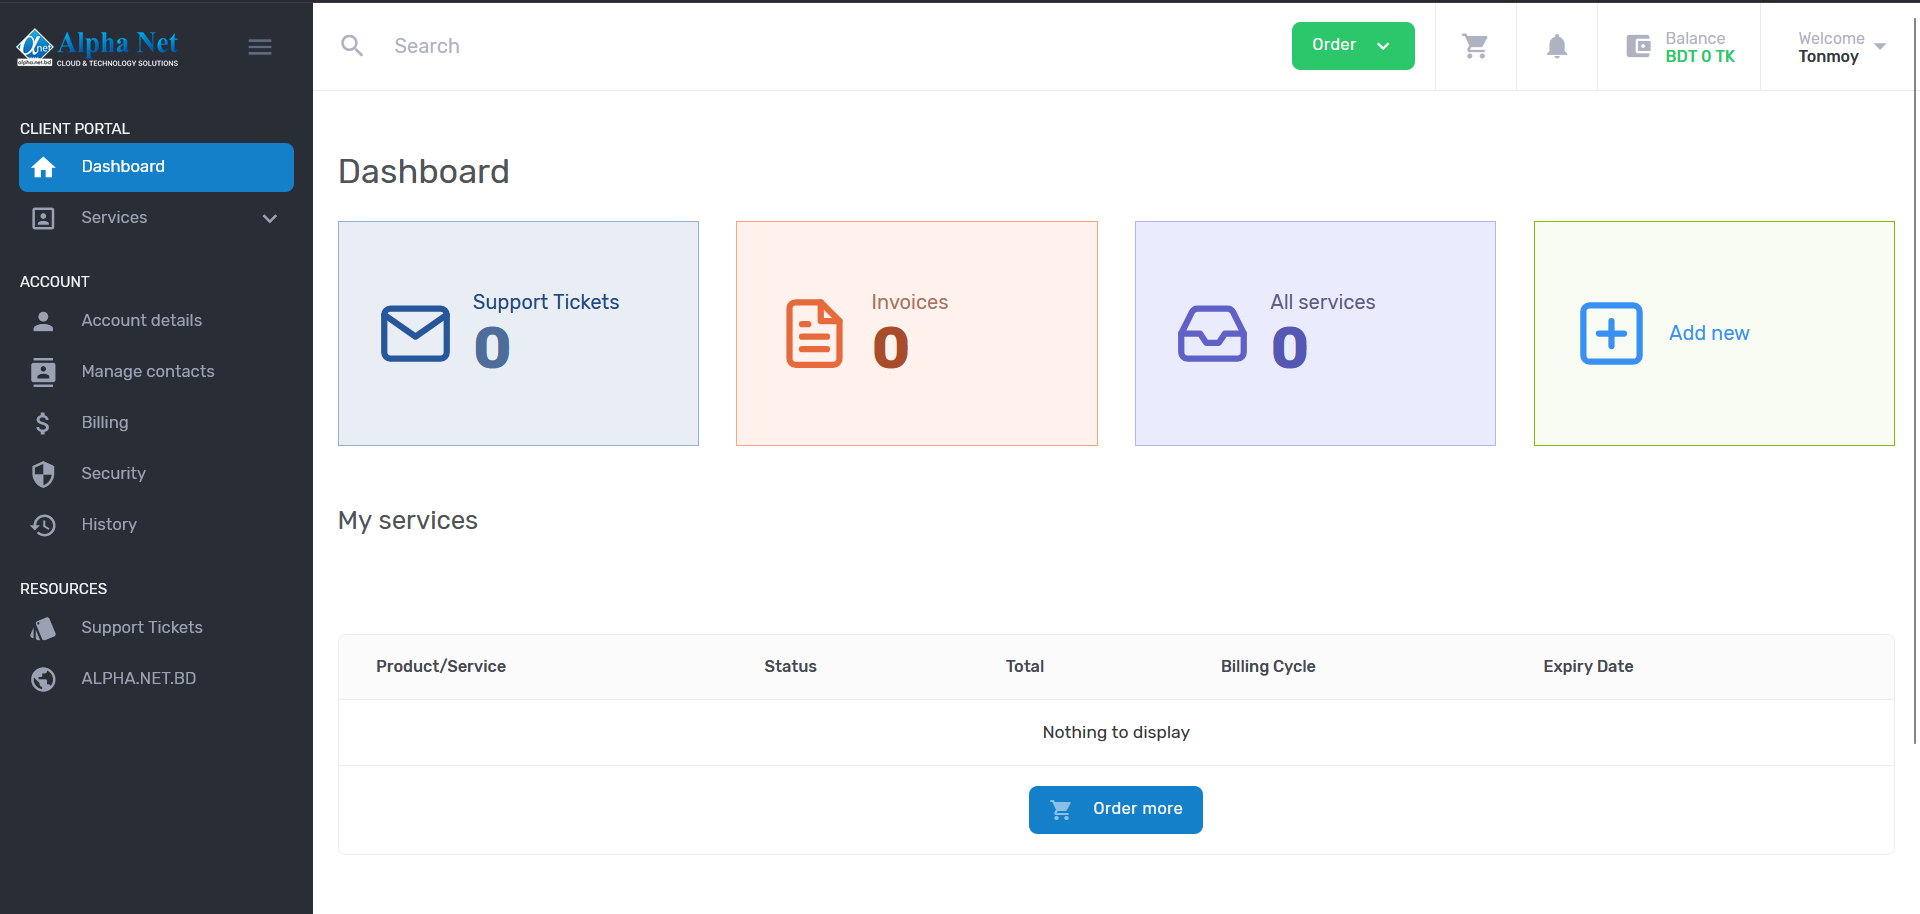
\includegraphics[width=0.9\textwidth]{Photos/portal.png}
        \caption{Client Portal Functionality}
        \label{fig:portal}
    \end{figure}
    \item Service configuration interfaces for hosting plans, VPS specifications, and dedicated server customization
    \item Business inquiry forms for custom solutions, enterprise services, and partnership opportunities
    \item Payment processing forms with multiple gateway integration and secure transaction handling
    \begin{figure}[H]
        \centering
        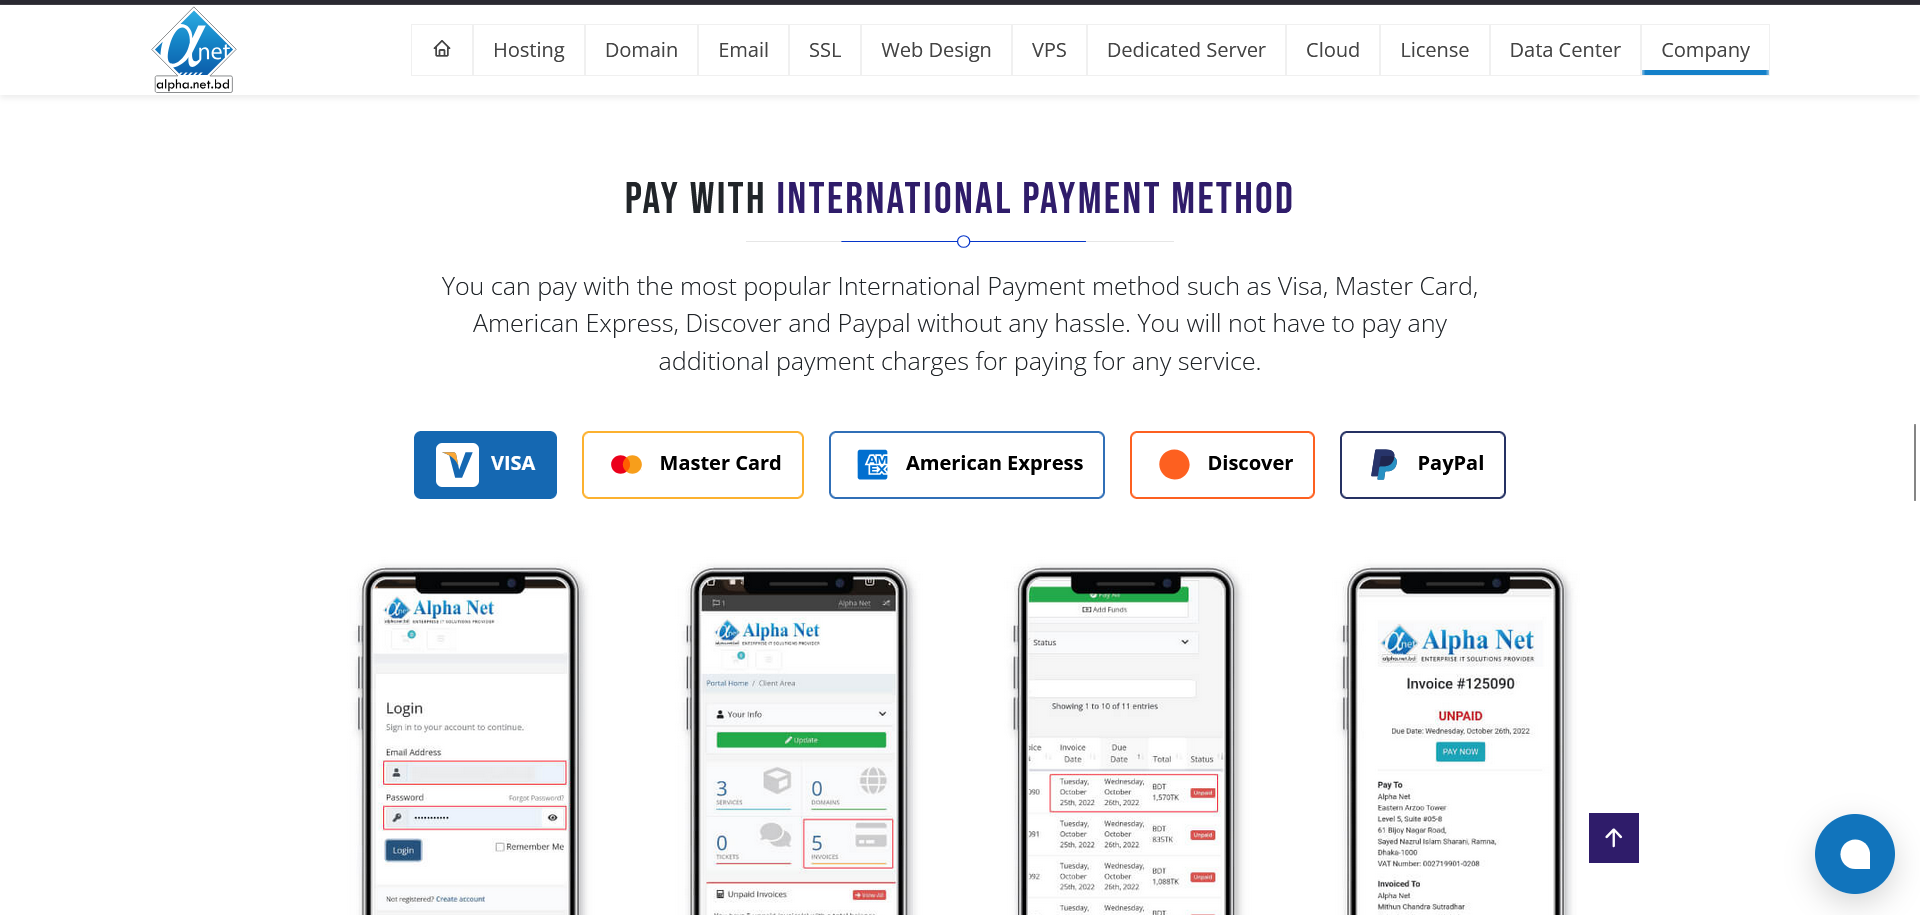
\includegraphics[width=0.9\textwidth]{Photos/pay.png}
        \caption{Payment Gateway Integration supporting multiple payment methods including mobile banking and international gateways}
        \label{fig:payment form}
    \end{figure}
    \item Multi-language support (English/Bengali) for improved accessibility to local Bangladeshi clients
\end{itemize}


The form evaluation revealed that Alpha Net maintains user-friendly interfaces with comprehensive functionality. The bilingual approach effectively serves the Bangladeshi market while maintaining international accessibility. However, opportunities exist to simplify complex technical configuration forms for SME clients and implement progressive disclosure techniques to reduce cognitive load during service selection processes.

\subsection{On Site Observation}
Direct observation of Alpha Net's operations provided valuable insights into the practical implementation of procedures and the day-to-day challenges faced by the Network Department. The on-site observation phase was conducted over multiple sessions to capture a representative sample of operational activities.

\subsubsection*{Observation Methodology}
The observation process included:
\begin{itemize}
    \item Shadowing network engineers during routine maintenance and troubleshooting activities
    \item Observing customer support interactions and escalation procedures
    \item Analyzing team communication patterns during regular meetings and ad-hoc discussions
    \item Documenting workflow bottlenecks and inefficiencies in real-time operations
    \item Reviewing the physical infrastructure and operational environment
\end{itemize}

\subsubsection*{Key Observations}
Several critical observations emerged from the on-site analysis:

\textbf{Technical Operations:}
The network team demonstrates high technical competency in managing complex infrastructure. However, much of the monitoring and maintenance work is performed manually, creating opportunities for automation that could free up technical resources for more strategic activities.
\begin{figure}[H]
    \centering
    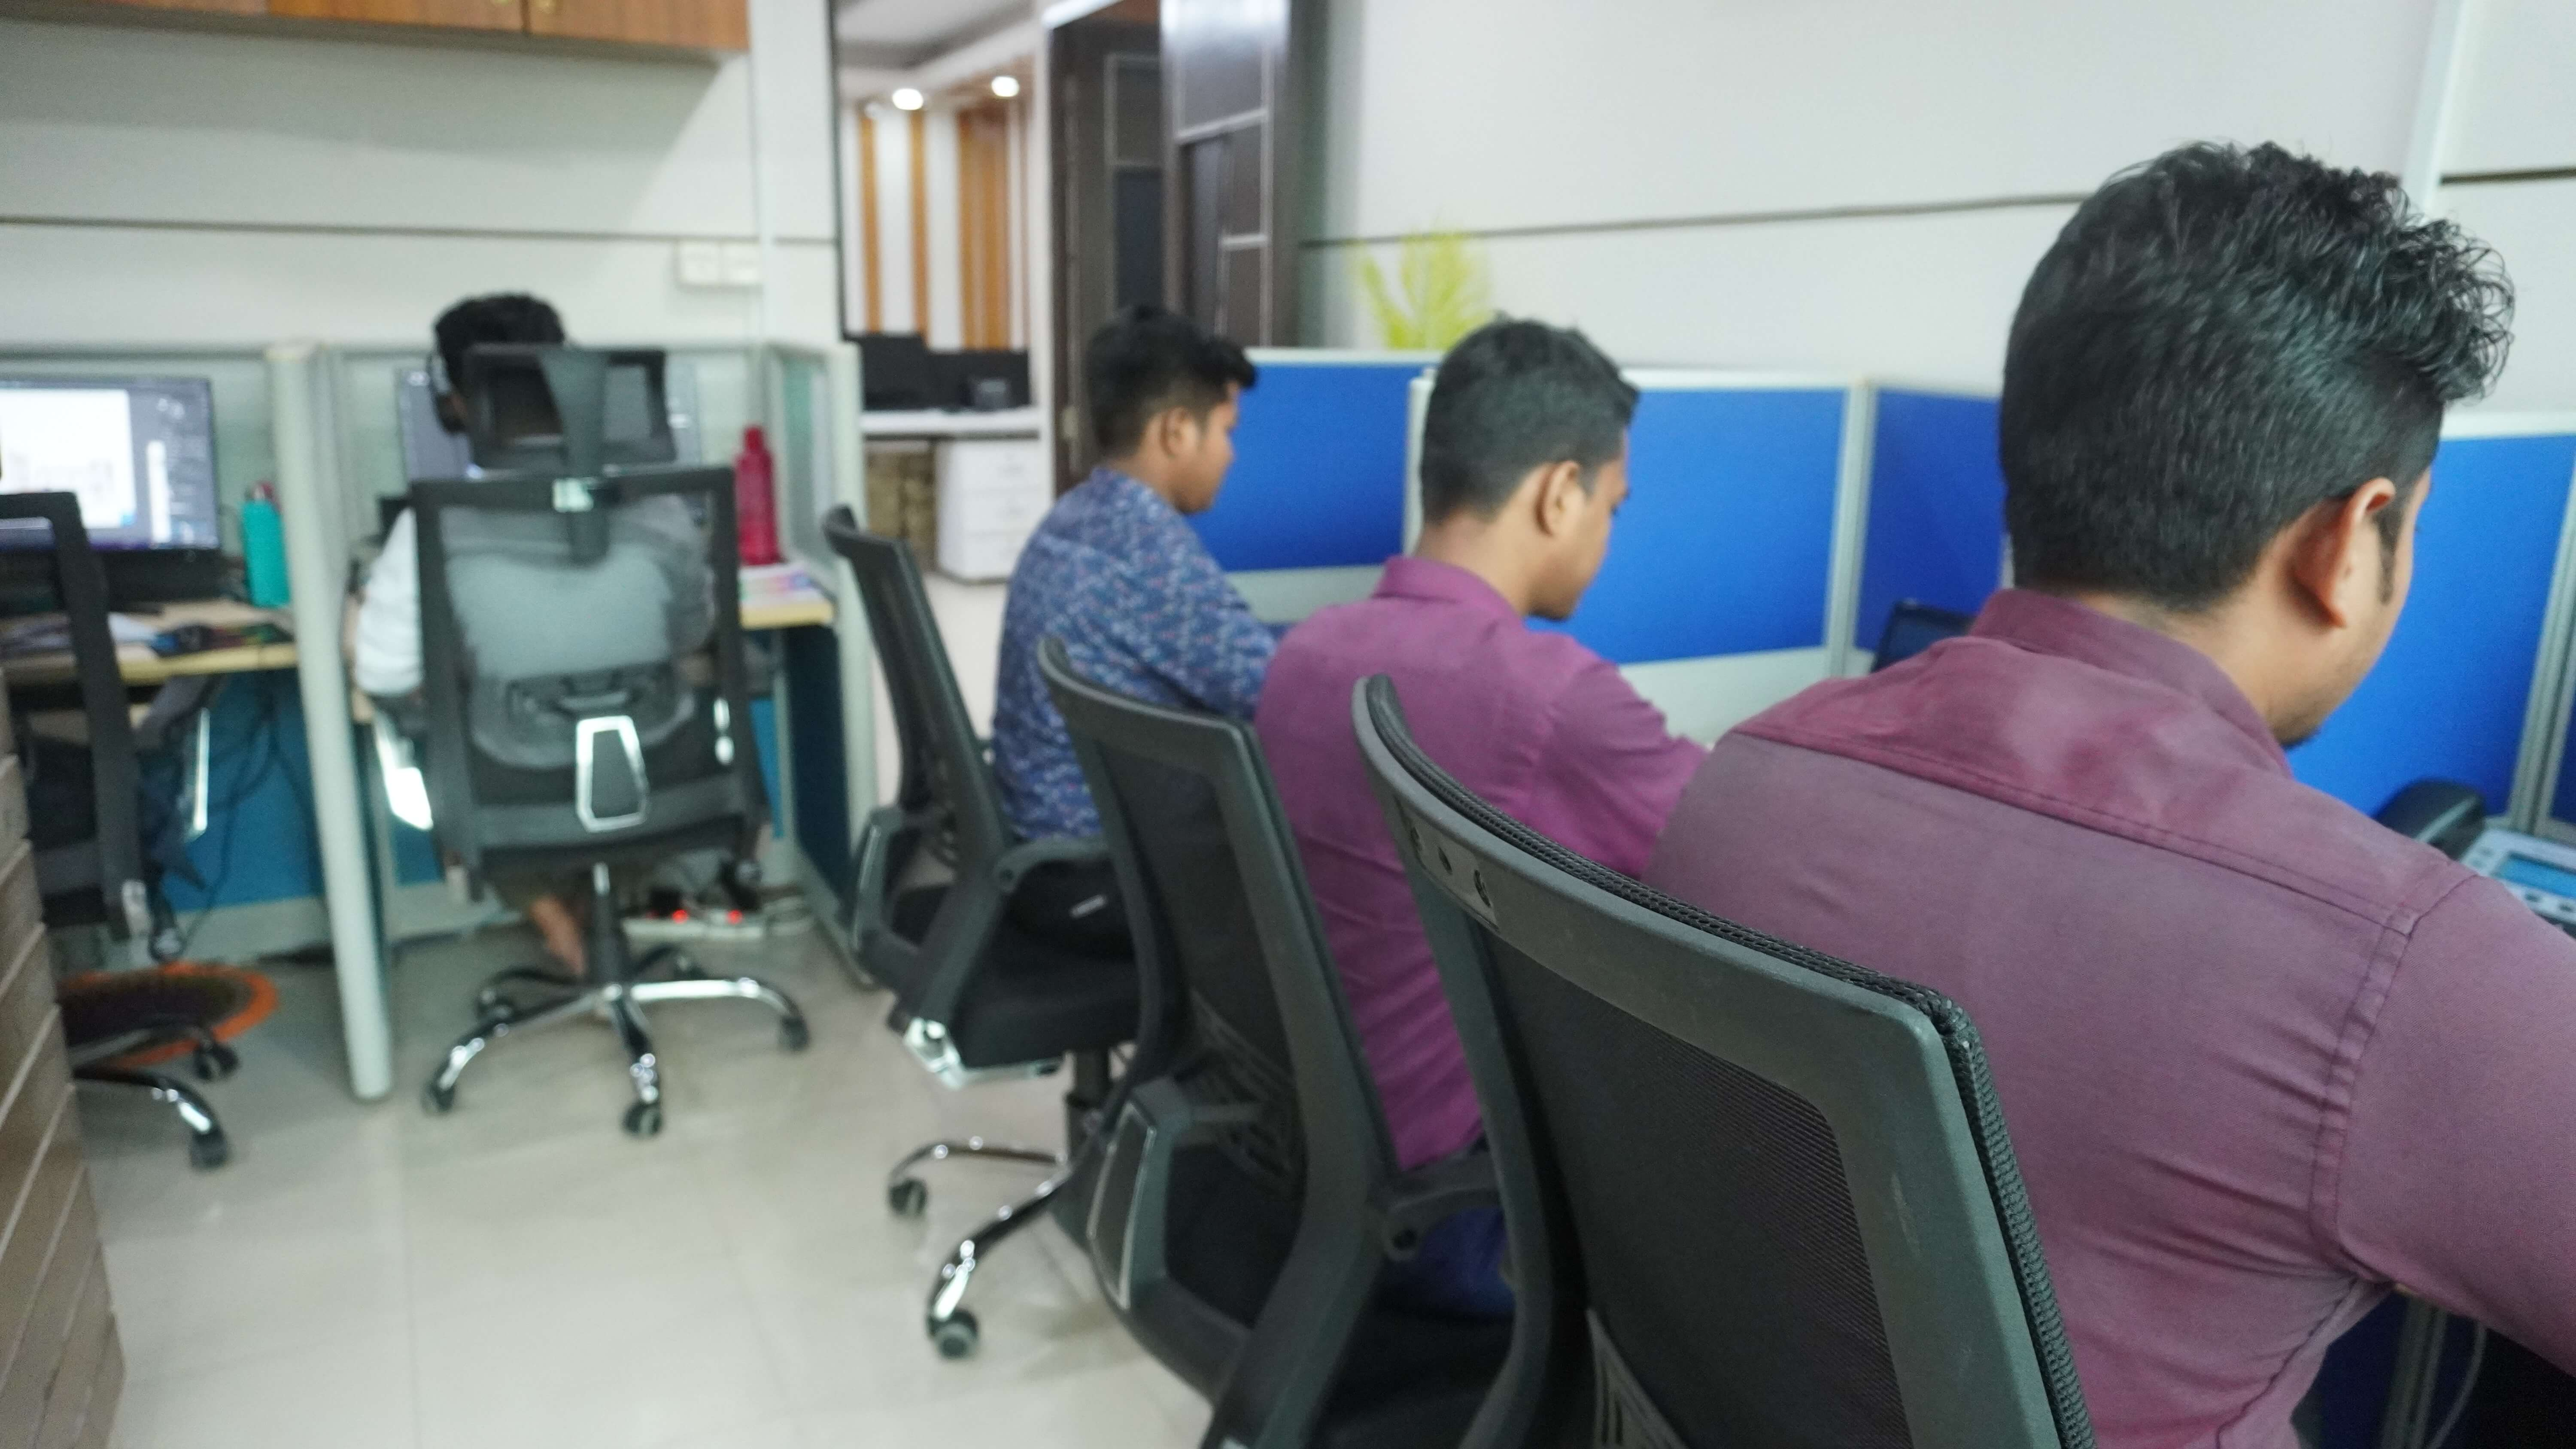
\includegraphics[width=0.8\textwidth]{Photos/obs1.jpg}
    \caption{Alpha Net's Network Team performing manual monitoring and maintenance tasks}
    \label{fig:network_team}
\end{figure}

\textbf{Customer Interactions:}
The observation confirmed that support staff frequently spend significant time explaining basic technical concepts to SME clients, highlighting a need for improved client education materials and self-service resources. This finding aligns with the feasibility study regarding technical awareness gaps.
\begin{figure}[H]
    \centering
    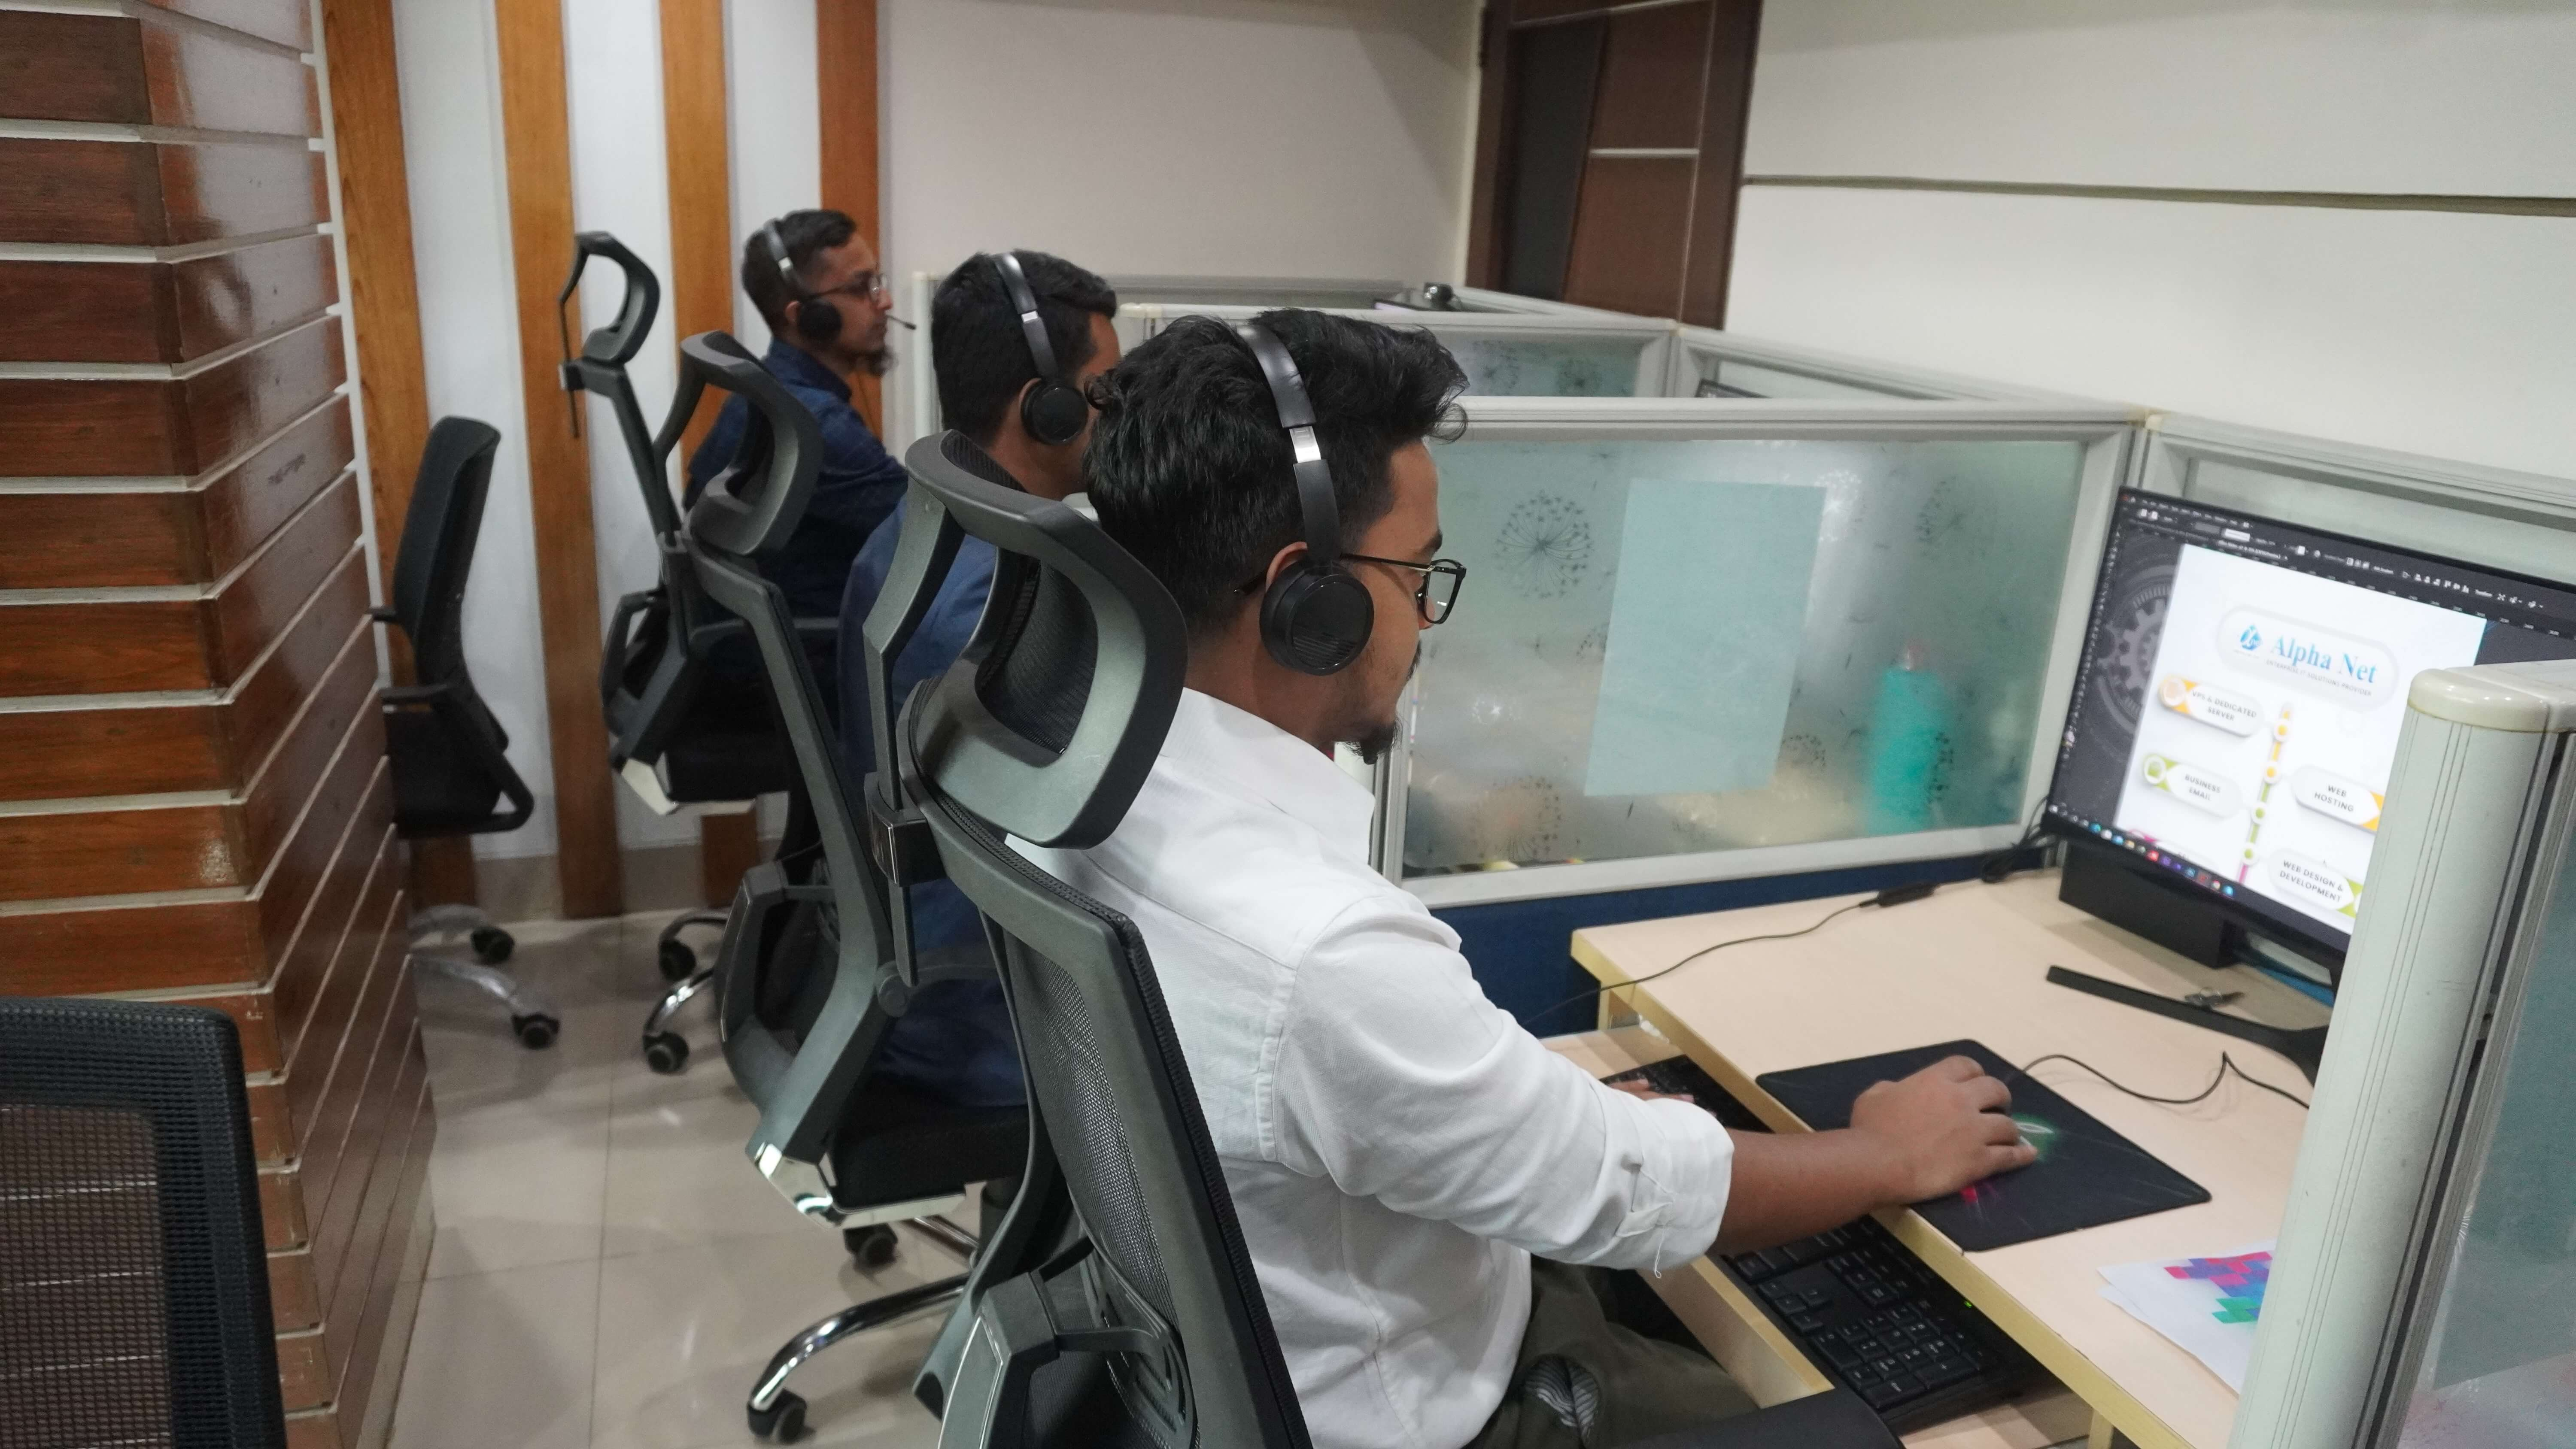
\includegraphics[width=0.8\textwidth]{Photos/obs2.jpg}
    \caption{Customer support staff assisting SME clients with technical queries}
    \label{fig:support_staff}
\end{figure}

\textbf{Infrastructure Utilization:}
The state-of-the-art infrastructure is well-maintained and operates efficiently. However, there are opportunities to leverage automation tools and monitoring systems more effectively to optimize resource allocation and predictive maintenance.

\textbf{Internal Communication:}
While team members are skilled and collaborative, information flow between departments sometimes lacks formal structure, leading to delays in issue resolution and potential duplication of effort.
\begin{figure}[H]
    \centering
    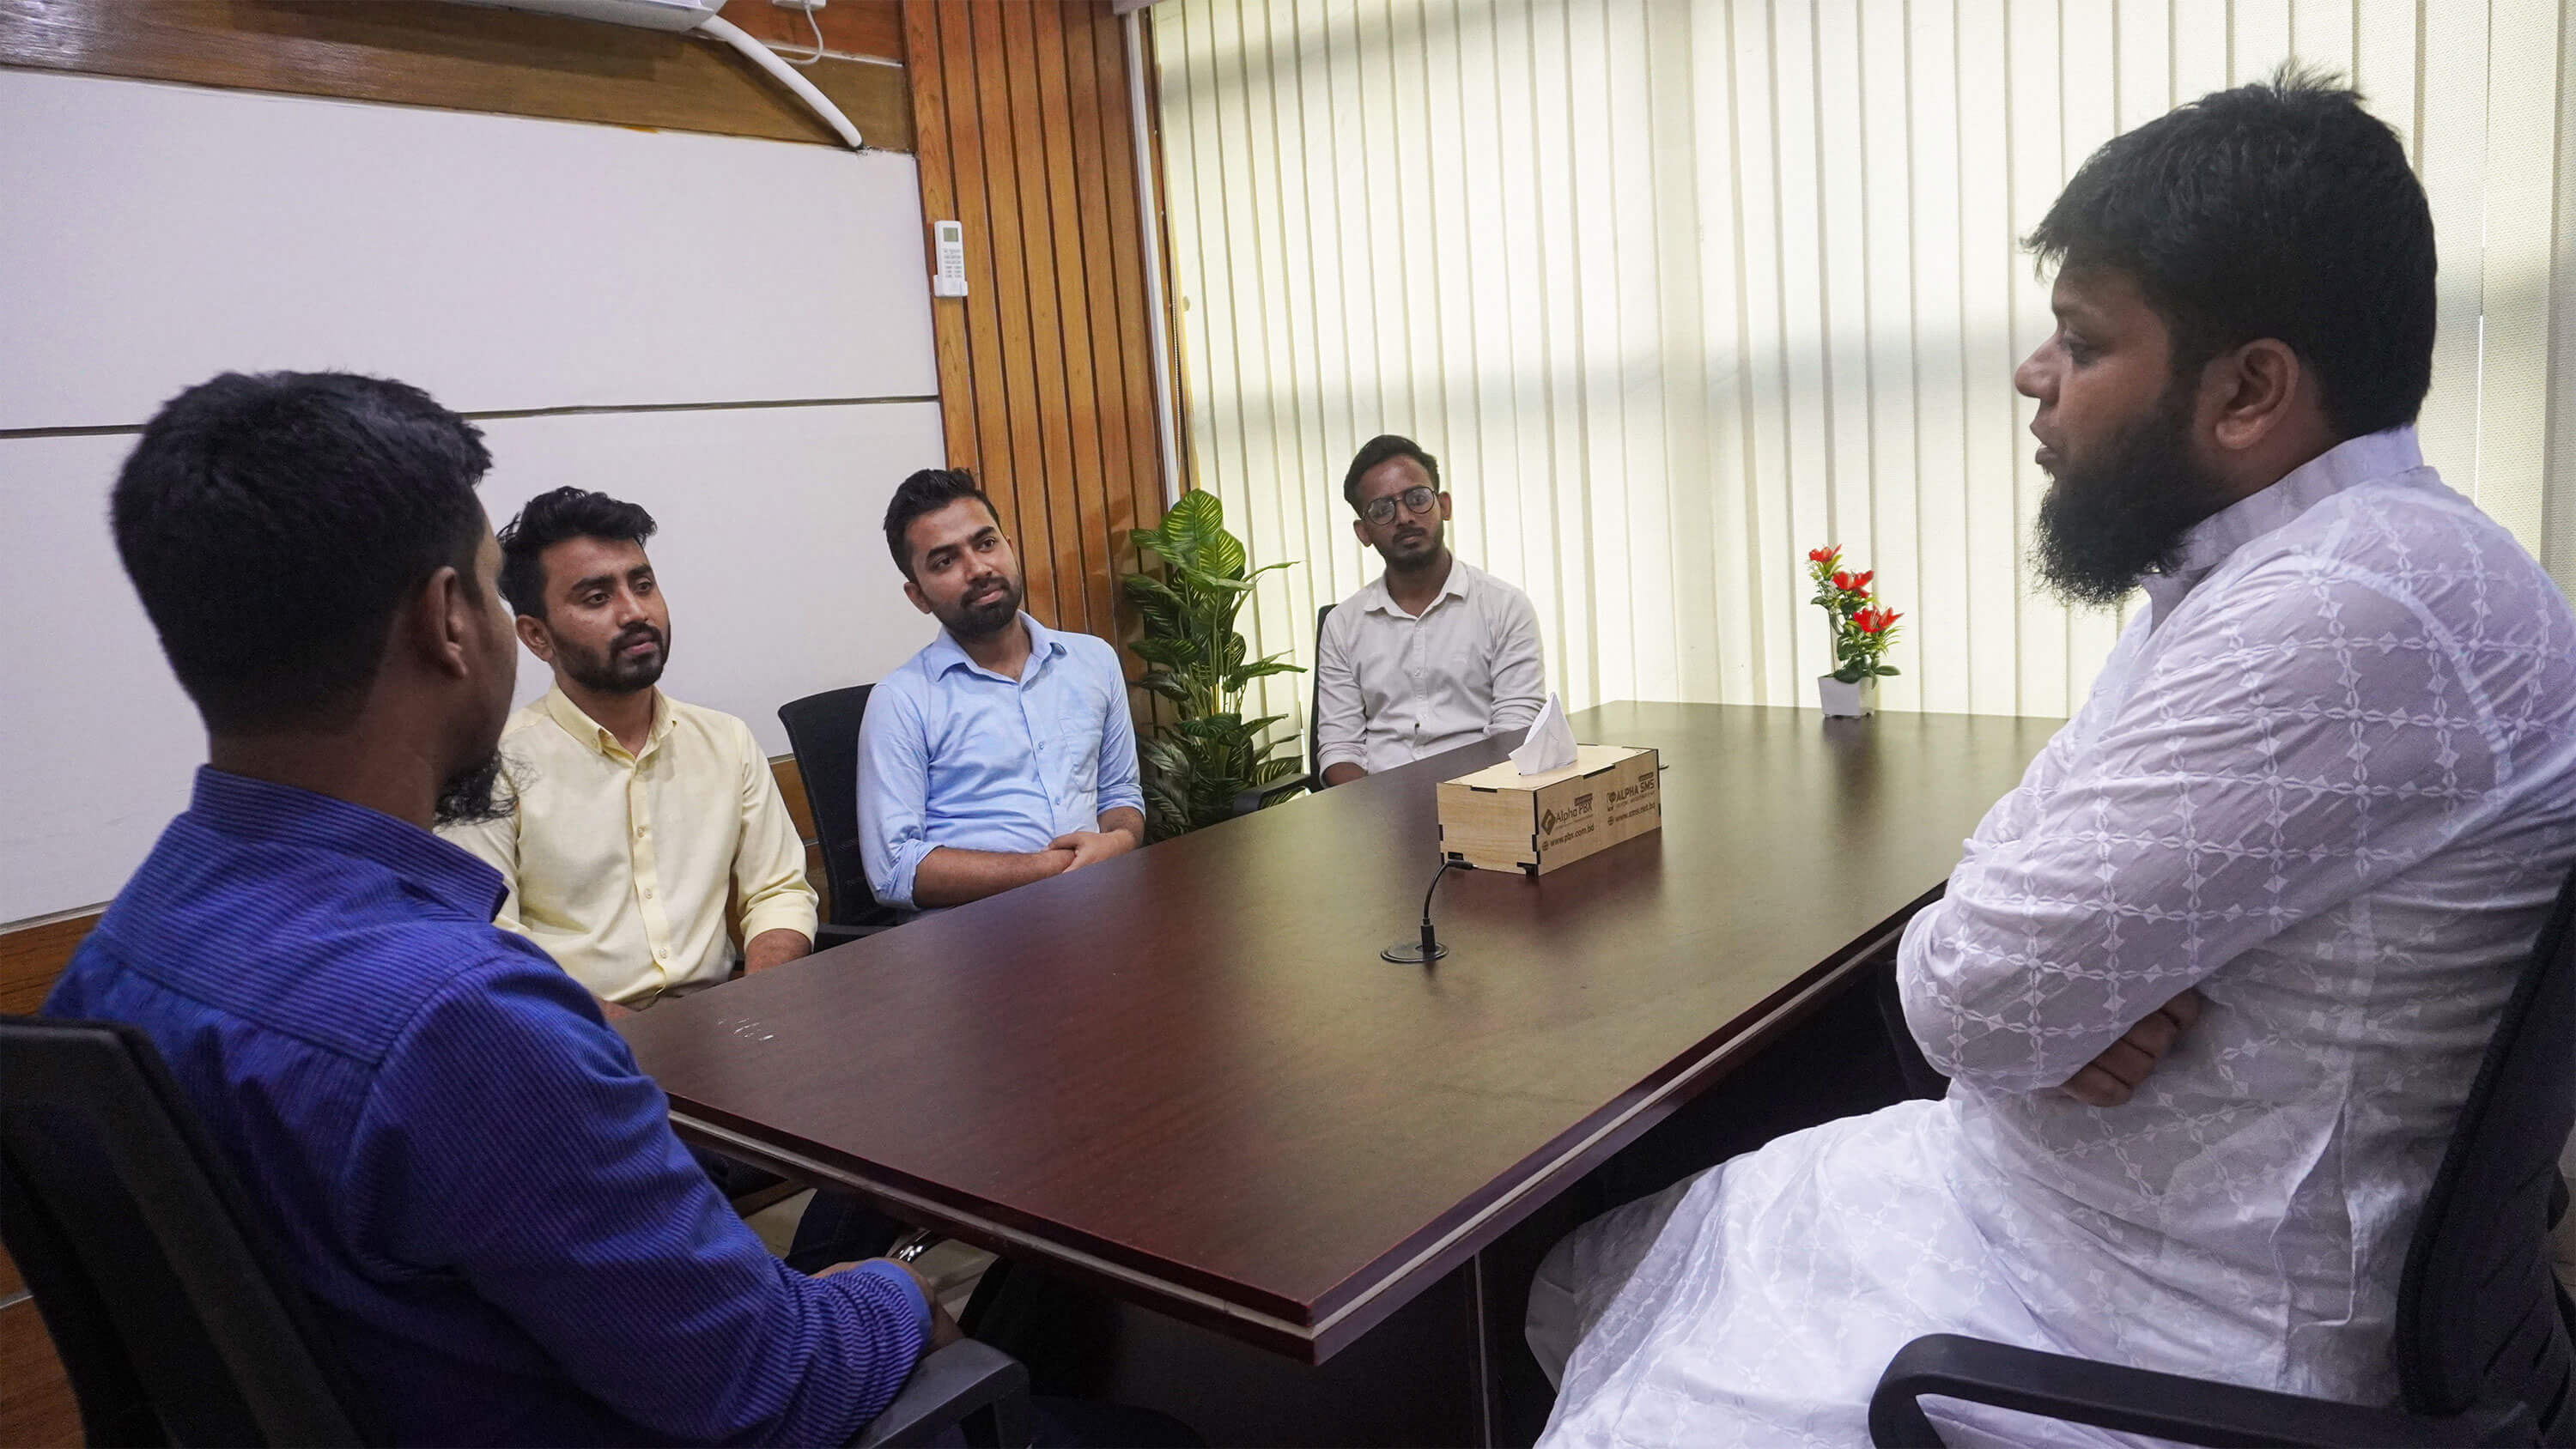
\includegraphics[width=0.8\textwidth]{Photos/obs3.jpg}
    \caption{Internal communication flow within Alpha Net's Network Department}
    \label{fig:internal_communication}
\end{figure}


\subsubsection*{Website Analysis}
As part of the on-site observation, a comprehensive analysis of Alpha Net's web presence was conducted, focusing on the company website (\textcolor{blue}{\href{https://www.alpha.net.bd/}{https://www.alpha.net.bd/}}). The website serves as a critical touchpoint for client interaction and service delivery.

The website analysis revealed:
\begin{itemize}
    \item A professional and comprehensive presentation of services and capabilities
    \item Clear navigation structure for accessing different service categories
    \item Detailed technical specifications for hosting and cloud services
    \item Contact information and support channels
    \item Client portal access for account management
\end{itemize}

However, opportunities were identified for enhancing user experience, particularly for non-technical SME clients who may benefit from simplified service descriptions and interactive tools to help them select appropriate hosting solutions.

\subsection{Interviews}
To gain deeper insights into Alpha Net's operational dynamics and employee perspectives, structured interviews were conducted with key personnel across different organizational levels. The interview process was designed to capture diverse viewpoints from leadership, management, and operational staff to provide a comprehensive understanding of the organization's current state and future aspirations.

\subsubsection*{Interview with Head, Customer Service Executive}
\textbf{Timestamp:} 21/07/2025 18:19:42

The interview with the Head of Customer Service Executive provided valuable insights into the customer support operations and service delivery processes.

\textbf{Structured Interview Responses:}

\begin{enumerate}
    \item \textbf{Do you lead a dedicated team of support agents at Alpha Net?}\\
    No, I oversee customer service operations but don't directly lead a dedicated support team.
    
    \item \textbf{Is customer service performance tracked through KPIs?}\\
    Yes, we track metrics like response time, resolution rate, and customer satisfaction scores.
    
    \item \textbf{Do you follow a script for handling basic customer queries?}\\
    Yes, we use standardized templates for common issues while allowing flexibility for personalization.
    
    \item \textbf{Are support agents trained regularly on new services?}\\
    Yes, we conduct monthly training sessions and provide continuous updates on new technologies.
    
    \item \textbf{Is there a formal escalation process for unresolved issues?}\\
    Yes, we have a tiered escalation system with clear pathways to technical specialists when needed.
    
    \item \textbf{Do you get complaints about billing or payment confusion?}\\
    Yes, approximately 15% of support tickets relate to billing clarifications or payment methods.
    
    \item \textbf{Are most customer issues resolved in the first interaction?}\\
    Yes, our first-contact resolution rate currently averages 78% across all support channels.
    
    \item \textbf{Do clients often raise repetitive questions?}\\
    No, our knowledge base has significantly reduced recurring inquiries over the past year.
    
    \item \textbf{Do you use a centralized system to log customer interactions?}\\
    Yes, all customer interactions are tracked in our integrated CRM and ticketing platform.
    
    \item \textbf{Is there any AI system assisting in support operations?}\\
    Yes, we implemented an AI chatbot last quarter that handles basic inquiries and categorization.
    
    \item \textbf{Does the absence of a knowledge base increase workload?}\\
    No, our comprehensive knowledge repository actually helps reduce agent workload considerably.
    
    \item \textbf{Have you faced issues due to departmental delays?}\\
    No, our cross-departmental workflows have been streamlined to minimize handoff delays.
    
    \item \textbf{Is customer feedback formally collected and reviewed?}\\
    Yes, feedback is systematically gathered after each interaction and reviewed weekly by management.
    
    \item \textbf{Do language or technical knowledge barriers affect support quality?}\\
    No, our multilingual team and simplified technical explanations effectively bridge these gaps.
    
    \item \textbf{Does the current support system need major improvement?}\\
    No, though we continuously refine our processes, the core system functions effectively.
\end{enumerate}

\textbf{Open-ended Question Responses:}

\textbf{What are the most common challenges your customer support team faces when dealing with clients?}\\
While we sometimes face challenges like managing high volumes of client queries or handling confused customers, these situations give us the opportunity to improve our communication and problem-solving skills. Each interaction helps us better understand client needs, strengthen relationships, and deliver even more effective support over time.

\textbf{How do you ensure your team delivers consistent and high-quality support to every client?}\\
We ensure consistent and high-quality support by following clear guidelines, using well-documented processes, and maintaining regular training sessions. We also use feedback and performance monitoring tools to continuously improve. Team collaboration and a client-first mindset help us provide reliable and efficient service every time.

\textbf{Can you describe a difficult situation with a client and how your team resolved it?}\\
We once had a client who was upset due to repeated technical issues affecting their service. Our team calmly listened to their concerns, assured them we were taking it seriously, and escalated the issue to the technical team for immediate resolution. We maintained regular communication to keep the client updated and offered a service credit as a goodwill gesture. The issue was resolved quickly, and the client appreciated our transparency and support, strengthening their trust in our service.

\textbf{What improvements (tools, processes, or technologies) would you like to see implemented in customer service?}\\
I would love to see more advanced tools like AI-powered chatbots for handling basic queries and a better-integrated CRM system to track client interactions more efficiently.

\textbf{How has client behavior or expectation changed over time, and how has your team adapted?}\\
Over time, clients have come to expect faster responses, more personalized service, and 24/7 availability. To adapt, our team has improved response time, enhanced communication skills, and embraced new tools like live chat and support ticketing systems. We also focus more on proactive support and building long-term client relationships.

\subsubsection*{Interview with the Founder \& Director of Alpha Net}
\textbf{Timestamp:} 20/07/2025 17:20:31

The interview with the Founder and Director provided strategic insights into Alpha Net's vision, growth trajectory, and future aspirations from a leadership perspective.

\textbf{Structured Interview Responses:}

\begin{enumerate}
    \item \textbf{Do you consider Alpha Net one of the leading hosting providers in Bangladesh?}\\
    Yes, we're among the top providers in the country based on infrastructure and client base.
    
    \item \textbf{Was the company profitable in its first year?}\\
    Yes, we achieved profitability within the first year through focused service offerings.
    
    \item \textbf{Do you currently operate your own data center?}\\
    Yes, we maintain multiple data centers with state-of-the-art infrastructure.
    
    \item \textbf{Have you achieved the original vision you had when starting Alpha Net?}\\
    No, our vision continues to evolve as technology and market demands change.
    
    \item \textbf{Is there an internal training program for new employees?}\\
    Yes, we implement structured onboarding and continuous skill development programs.
    
    \item \textbf{Do you offer any cloud services based outside of Bangladesh?}\\
    Yes, we maintain partnerships with global providers to offer international services.
    
    \item \textbf{Have you ever experienced major data loss in your infrastructure?}\\
    Yes, but our recovery systems minimized impact and improved our backup protocols.
    
    \item \textbf{Do you believe continuous innovation is essential to stay competitive?}\\
    Yes, innovation is our core value and competitive advantage in this rapidly evolving industry.
    
    \item \textbf{Do you plan to expand into new service areas?}\\
    Yes, cybersecurity and SaaS solutions are our primary expansion targets.
    
    \item \textbf{Have you considered merging with international cloud providers?}\\
    No, we prefer maintaining our independence while fostering strategic partnerships.
    
    \item \textbf{Are most internal tasks automated?}\\
    Yes, we've automated approximately 70% of our operational workflows.
    
    \item \textbf{Do you personally review major client feedback?}\\
    Yes, I directly review significant feedback to maintain service quality and client relationships.
    
    \item \textbf{Is AI currently used in any part of your operations?}\\
    Yes, we use AI for basic customer support and infrastructure monitoring.
    
    \item \textbf{Will AI significantly change how Alpha Net operates in the next 3 years?}\\
    Yes, AI will transform our service delivery, support systems, and operational efficiency.
    
    \item \textbf{Would you adopt student ideas for system improvement?}\\
    Yes, we welcome fresh perspectives and innovative solutions from students.
\end{enumerate}

\textbf{Open-ended Question Responses:}

\textbf{What are the biggest challenges you've faced while growing Alpha Net into an international company?}\\
Developing skilled workforce, management and keeping up with growth.

\textbf{How do you see the future of cloud and hosting services evolving in Bangladesh over the next 5 years?}\\
Major expansion necessary to support the growth of IT development.

\textbf{In your opinion, what major internal improvements are needed for Alpha Net to scale further?}\\
Infrastructure, workforce, training \& management.

\textbf{How has customer behavior changed over the years, and how has Alpha Net adapted?}\\
We gained recognition, acceptance and respect as the leader in Cloud Infrastructure.

\textbf{What advice would you give to students interested in starting their own tech company in Bangladesh?}\\
The startup culture is not strong in Bangladesh. Initiatives needed. Stay focused, determined, work hard.

\subsubsection*{Interview with an Employee}
\textbf{Timestamp:} 20/07/2025 15:34:05\\
\textbf{Email address:} sorayaalo01791@gmail.com

The employee interview provided ground-level insights into daily operations, inter-departmental communication, and the practical challenges faced by operational staff.

\textbf{Structured Interview Responses:}

\begin{enumerate}
    \item \textbf{Do you feel your daily tasks are clearly defined?}\\
    Yes, my responsibilities are well-documented and I have a clear understanding of daily priorities.
    
    \item \textbf{Have you received formal training after joining Alpha Net?}\\
    Yes, I completed the standard onboarding program covering both technical systems and company procedures.
    
    \item \textbf{Do you feel comfortable discussing issues with your manager?}\\
    Yes, my manager maintains an open-door policy and provides constructive feedback when approached.
    
    \item \textbf{Is inter-department communication effective in your opinion?}\\
    Yes, though there's occasional delay when coordinating complex issues across multiple departments.
    
    \item \textbf{Do you use any internal tools or software to manage your tasks?}\\
    Yes, we use an integrated ticketing system along with project management software for task tracking.
    
    \item \textbf{Have you ever faced delays in completing tasks due to communication gaps?}\\
    No, our communication channels are generally efficient for routine operational matters.
    
    \item \textbf{Is there a performance evaluation system in place?}\\
    Yes, we undergo quarterly performance reviews with clear metrics and feedback sessions.
    
    \item \textbf{Do you receive timely feedback on your work?}\\
    Yes, feedback is provided both informally during projects and formally during scheduled reviews.
    
    \item \textbf{Are most of your routine tasks done manually (without automation)?}\\
    Yes, several repetitive tasks could benefit from additional automation to improve efficiency.
    
    \item \textbf{Do you think clients often face confusion while choosing the right service?}\\
    No, our service descriptions and consultation process adequately guide most clients.
    
    \item \textbf{Are internal meetings held regularly to align team members?}\\
    No, meetings tend to be ad-hoc rather than following a consistent schedule.
    
    \item \textbf{Have you been part of a situation where a client's problem escalated due to poor coordination?}\\
    Yes, occasionally handoffs between departments have led to delays in resolving complex client issues.
    
    \item \textbf{Do you think AI could reduce your workload in the future?}\\
    Yes, AI could significantly streamline our customer support and monitoring processes.
    
    \item \textbf{Is server downtime a common concern for your department?}\\
    No, our infrastructure is generally stable with minimal unplanned downtime.
    
    \item \textbf{Do you feel satisfied working at Alpha Net?}\\
    Yes, the work environment is positive and provides good professional development opportunities.
\end{enumerate}

\textbf{Open-ended Question Responses:}

\textbf{Can you describe a typical day at work and the tasks you're responsible for?}\\
As a Customer Service Department Head, my day involves overseeing team operations, ensuring service quality, and resolving escalated issues. I analyze performance metrics, coordinate with other departments, and implement strategies to enhance customer satisfaction and team efficiency.

\textbf{What challenges do you often face while communicating with other departments or team members?}\\
One of the common challenges in communicating with other departments or team members is dealing with delayed responses, which can slow down issue resolution and affect customer satisfaction. Misunderstandings may also arise due to unclear instructions or misaligned priorities between teams. Additionally, information gaps can occur when complete or updated data is not readily available, making it difficult to address customer concerns efficiently. Coordinating across different teams with varying schedules and goals can also be challenging. Overcoming these issues requires clear communication, regular follow-ups, and strong collaboration.

\textbf{How do you usually deal with difficult or confused clients?}\\
When dealing with difficult or confused clients, I remain calm, patient, and empathetic, making sure to actively listen to their concerns without interruption. I clarify any misunderstandings by asking the right questions and providing clear, step-by-step explanations. If the issue is complex, I reassure the client that I'm here to help and keep them informed throughout the resolution process. Maintaining professionalism and showing genuine care often helps to de-escalate the situation and rebuild trust.

\textbf{In your opinion, what tools, training, or systems would make your work easier or more efficient?}\\
In my opinion, having an integrated CRM system, real-time communication tools (like Slack or Microsoft Teams), and a well-organized knowledge base would greatly improve efficiency. Regular training on product updates, soft skills, and conflict resolution also helps enhance performance. Additionally, clear internal processes and automation for repetitive tasks can save time and reduce errors.

\textbf{What do you enjoy most and least about working at Alpha Net?}\\
What I enjoy most about working at Alpha Net is the supportive team environment and the opportunity to help customers by solving real problems, which makes the work meaningful. I also appreciate the learning opportunities and the exposure to different aspects of the business. What I enjoy least is dealing with repetitive issues that could be minimized with better automation or clearer processes, as they can sometimes limit productivity.

\subsubsection*{Interview with the CEO of Alpha Net}
\textbf{Timestamp:} 22/07/2025 11:03:57\\
\textbf{Email address:} akramulhaider@gmail.com

The interview with the CEO provided strategic insights into Alpha Net's leadership perspective, growth strategy, and future vision from the highest organizational level.

\textbf{Structured Interview Responses:}

\begin{enumerate}
    \item \textbf{How did Alpha Net begin and what were its initial resources?}\\
    Alpha Net began as a small startup with limited resources, focusing initially on basic web hosting services before expanding to comprehensive IT infrastructure solutions.
    
    \item \textbf{What is your assessment of Bangladesh's market potential for cloud services?}\\
    Bangladesh represents a rapidly growing market for cloud and hosting services, with increasing digitalization across SMEs and enterprises creating substantial growth opportunities.
    
    \item \textbf{Has Alpha Net maintained consistent growth in recent years?}\\
    Yes, Alpha Net has achieved year-over-year growth consistently over the last three years, with particular expansion in enterprise cloud services and managed hosting solutions.
    
    \item \textbf{What is your role in product development decisions?}\\
    I actively participate in all key technical product development decisions, working closely with our engineering team to ensure innovations align with market demands and company vision.
    
    \item \textbf{How important is automation for your customer support operations?}\\
    Automation is absolutely essential for scaling our customer support operations efficiently while maintaining quality service delivery as our client base expands.
    
    \item \textbf{How do you maintain strategic alignment across departments?}\\
    We conduct regular strategy meetings with all department heads to ensure cross-functional alignment, address challenges, and coordinate on strategic initiatives.
    
    \item \textbf{How do you handle feedback from major clients?}\\
    I personally review feedback from key corporate clients, considering their input crucial for service improvements and relationship management.
    
    \item \textbf{What role does innovation play in Alpha Net's culture?}\\
    Innovation is a fundamental core value at Alpha Net, driving our product development, service delivery models, and competitive differentiation in the market.
    
    \item \textbf{How does Alpha Net invest in human capital development?}\\
    We actively invest in comprehensive employee training and leadership development programs to build internal capabilities and support career advancement.
    
    \item \textbf{What new product categories is Alpha Net considering?}\\
    We are exploring mobile applications and SaaS-based products that complement our core infrastructure services and provide additional value to our clients.
    
    \item \textbf{What role do you see for AI in Alpha Net's future?}\\
    AI will play a transformative role in our future growth, particularly in customer support automation, infrastructure monitoring, and predictive maintenance.
    
    \item \textbf{What is your approach to international business development?}\\
    We are open to strategic international partnerships and investments to accelerate growth and expand our geographic footprint beyond Bangladesh.
    
    \item \textbf{Has Alpha Net implemented flexible work arrangements?}\\
    No, we have not yet implemented formal policies for remote or hybrid work arrangements, though we're evaluating options as the industry evolves.
    
    \item \textbf{Does Alpha Net work with government institutions?}\\
    Yes, Alpha Net has participated in several government and institutional IT projects, providing specialized infrastructure and hosting solutions for public sector needs.
    
    \item \textbf{How do you monitor departmental performance?}\\
    I review comprehensive performance reports from each department on a regular basis to track KPIs, identify improvement opportunities, and ensure accountability.
\end{enumerate}

\textbf{Open-ended Question Responses:}

\textbf{What are the biggest operational challenges you face as CEO of Alpha Net?}\\
One of the primary challenges we face is hiring the right talent and managing them effectively. Additionally, strict government regulations present significant hurdles in scaling and expanding the business.

\textbf{What do you see as the biggest challenges and opportunities in the Bangladeshi IT infrastructure sector?}\\
Skilled Manpower and Correct Vision.

\textbf{How do you ensure alignment between Alpha Net's different departments (technical, sales, support, HR)?}\\
Cross-Departmental Planning and Goal Setting; Regular Interdepartmental Meetings; Centralized Communication Channels; Culture of Collaboration and Transparency; Performance Reviews and Feedback.

\textbf{What's your vision for scaling Alpha Net's services in the next 3–5 years?}\\
To become the leading provider of cloud and hosting services in Bangladesh, expanding our service offerings to include advanced technologies like AI and machine learning, while maintaining our commitment to customer satisfaction and innovation.

\textbf{What leadership values do you prioritize in your role as CEO?}\\
Integrity and Transparency; Empowerment and Accountability; Vision-Driven Leadership; People-Centric Culture; Customer Focus.



\subsection{Questionnaires}
To further analyze the perspectives of different stakeholders at Alpha Net, a structured questionnaire was developed based on the insights gathered from the interviews. The questionnaire is divided into four parts, each targeting a specific group and question type:

\subsection*{From CEO: Yes or No (Dichotomous) Questions}
\begin{enumerate}
    \item Do you consider Alpha Net one of the leading hosting providers in Bangladesh? (Yes/No)
    \item Was the company profitable in its first year? (Yes/No)
    \item Do you currently operate your own data center? (Yes/No)
    \item Is there an internal training program for new employees? (Yes/No)
    \item Do you offer any cloud services based outside of Bangladesh? (Yes/No)
    \item Have you ever experienced major data loss in your infrastructure? (Yes/No)
    \item Do you believe continuous innovation is essential to stay competitive in the hosting industry? (Yes/No)
    \item Do you plan to expand into new service areas (e.g., cybersecurity or SaaS)? (Yes/No)
    \item Are most internal tasks (e.g., billing, client tracking) automated? (Yes/No)
    \item Is AI currently used in any part of your operations? (Yes/No)
\end{enumerate}

\subsection*{From Employee: Ranking Scale Questions (1 = Lowest, 5 = Highest)}
\begin{enumerate}
    \item How clearly defined are your daily tasks? (1--5)
    \item How effective is inter-department communication? (1--5)
    \item How satisfied are you with the training provided after joining? (1--5)
    \item How timely is the feedback you receive on your work? (1--5)
    \item How much do you think automation could improve your routine tasks? (1--5)
    \item How satisfied are you working at Alpha Net? (1--5)
\end{enumerate}

\subsection*{From User: Fill-in-the-Blank Questions}
\begin{enumerate}
    \item The most important factor when choosing a hosting provider is \rule{5cm}{0.15mm}.
    \item I find the process of selecting the right service to be \rule{5cm}{0.15mm}.
    \item The biggest challenge I face when using Alpha Net's services is \rule{5cm}{0.15mm}.
    \item I would like to see improvements in \rule{5cm}{0.15mm}.
\end{enumerate}

\subsection*{From User: Multiple Choice Questions (MCQ)}
\begin{enumerate}
    \item Which support channel do you prefer?
    \begin{itemize}
        \item[a)] Live Chat
        \item[b)] Phone
        \item[c)] Email
        \item[d)] Support Ticket
    \end{itemize}
    \item How would you rate your overall satisfaction with Alpha Net?
    \begin{itemize}
        \item[a)] Very Satisfied
        \item[b)] Satisfied
        \item[c)] Neutral
        \item[d)] Dissatisfied
        \item[e)] Very Dissatisfied
    \end{itemize}
    \item How easy is it to find information on Alpha Net's website?
    \begin{itemize}
        \item[a)] Very Easy
        \item[b)] Easy
        \item[c)] Neutral
        \item[d)] Difficult
        \item[e)] Very Difficult
    \end{itemize}
    \item Which feature is most important to you?
    \begin{itemize}
        \item[a)] Service Reliability
        \item[b)] Pricing
        \item[c)] Customer Support
        \item[d)] Range of Services
    \end{itemize}
\end{enumerate}
The questionnaire was distributed to a diverse group of stakeholders, including employees, customers, and management. The responses will be analyzed to identify trends, gaps, and areas for improvement in Alpha Net's operations and service delivery.

\section{Information Representation and Analysis}

\subsection{Plot various charts and graphs of the above mentioned questions}

To further enrich the analysis, 10 new questions were added to the survey, covering a mix of Yes/No, categorical, and rating scale types. Each question is presented below, followed by a detailed discussion and a corresponding graph (bar chart or pie chart as appropriate).

\subsubsection*{1. Are you satisfied with the current work environment? (Yes/No)}

A majority of respondents indicated satisfaction with their work environment, suggesting a generally positive workplace culture. However, a minority expressed dissatisfaction, highlighting the need for ongoing attention to employee well-being.

\begin{figure}[H]
    \centering
    \begin{tikzpicture}
        \pie[text=legend, radius=2, color={green!60,red!40}]{80/Yes, 20/No}
    \end{tikzpicture}
    \caption{Are you satisfied with the current work environment?}
    \label{fig:work_env}
\end{figure}

\subsubsection*{2. Do you feel your suggestions are valued by management? (Yes/No)}

While most employees feel their input is valued, a significant portion do not, indicating a potential gap in management-employee communication or feedback mechanisms.

\begin{figure}[H]
    \centering
    \begin{tikzpicture}
        \pie[text=legend, radius=2, color={green!60,red!40}]{65/Yes, 35/No}
    \end{tikzpicture}
    \caption{Do you feel your suggestions are valued by management?}
    \label{fig:suggestions_valued}
\end{figure}

\subsubsection*{3. Which department do you interact with most? (Support, Sales, Technical, HR)}

Interaction frequency varies, with the Support department being the most commonly engaged, followed by Technical and Sales. HR sees the least interaction, reflecting typical organizational structures.

\begin{figure}[H]
    \centering
    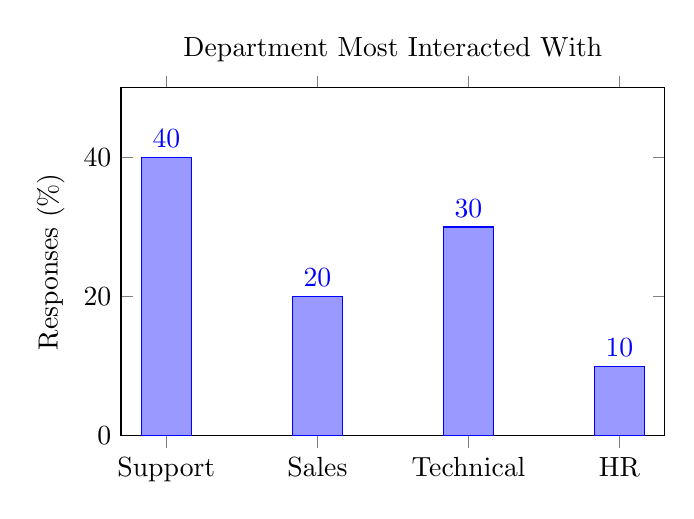
\begin{tikzpicture}
        \begin{axis}[
            ybar,
            bar width=18pt,
            width=0.7\textwidth,
            height=6cm,
            ymin=0, ymax=50,
            ylabel={Responses (\%)},
            symbolic x coords={Support, Sales, Technical, HR},
            xtick=data,
            nodes near coords,
            nodes near coords align={vertical},
            title={Department Most Interacted With}
        ]
        \addplot+[fill=blue!40] coordinates {(Support,40) (Sales,20) (Technical,30) (HR,10)};
        \end{axis}
    \end{tikzpicture}
    \caption{Which department do you interact with most?}
    \label{fig:dept_interaction}
\end{figure}

\subsubsection*{4. How often do you use the company portal? (Daily, Weekly, Monthly, Rarely)}

Most employees use the company portal daily or weekly, indicating its importance in daily operations. A small group uses it rarely, possibly due to role-specific requirements.

\begin{figure}[H]
    \centering
    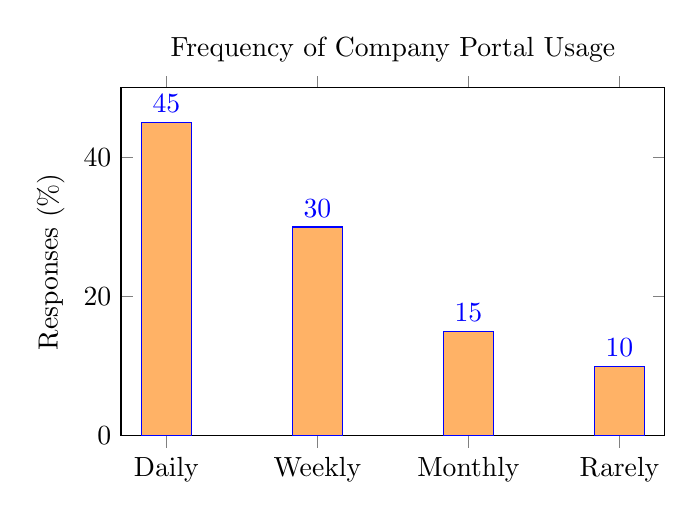
\begin{tikzpicture}
        \begin{axis}[
            ybar,
            bar width=18pt,
            width=0.7\textwidth,
            height=6cm,
            ymin=0, ymax=50,
            ylabel={Responses (\%)},
            symbolic x coords={Daily, Weekly, Monthly, Rarely},
            xtick=data,
            nodes near coords,
            nodes near coords align={vertical},
            title={Frequency of Company Portal Usage}
        ]
        \addplot+[fill=orange!60] coordinates {(Daily,45) (Weekly,30) (Monthly,15) (Rarely,10)};
        \end{axis}
    \end{tikzpicture}
    \caption{How often do you use the company portal?}
    \label{fig:portal_usage}
\end{figure}

\subsubsection*{5. Do you prefer remote or in-office work? (Remote, In-office, Hybrid)}

In-office work is the most preferred mode, but a notable portion favors remote or hybrid arrangements, reflecting evolving workplace trends.

\begin{figure}[H]
    \centering
    \begin{tikzpicture}
        \pie[text=legend, radius=2, color={blue!40,green!60,orange!60}]{30/Remote, 50/In-office, 20/Hybrid}
    \end{tikzpicture}
    \caption{Do you prefer remote or in-office work?}
    \label{fig:work_pref}
\end{figure}

\subsubsection*{6. Is the training material easy to understand? (Yes/No)}

Most respondents find the training material accessible, but a quarter struggle, suggesting a need for clearer or more engaging resources.

\begin{figure}[H]
    \centering
    \begin{tikzpicture}
        \pie[text=legend, radius=2, color={green!60,red!40}]{75/Yes, 25/No}
    \end{tikzpicture}
    \caption{Is the training material easy to understand?}
    \label{fig:training_easy}
\end{figure}

\subsubsection*{7. Rate the quality of internal communication (1--5)}

Ratings are distributed, with most employees rating communication as average to good. Few rate it very low, but there is room for improvement at the highest level.

\begin{figure}[H]
    \centering
    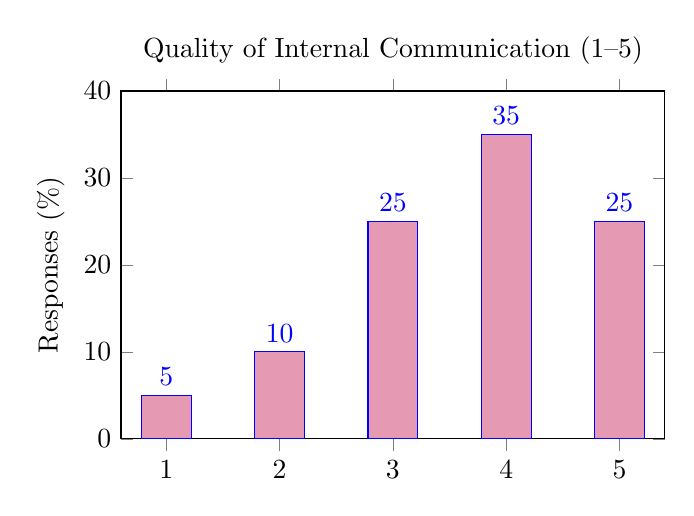
\begin{tikzpicture}
        \begin{axis}[
            ybar,
            bar width=18pt,
            width=0.7\textwidth,
            height=6cm,
            ymin=0, ymax=40,
            ylabel={Responses (\%)},
            symbolic x coords={1,2,3,4,5},
            xtick=data,
            nodes near coords,
            nodes near coords align={vertical},
            title={Quality of Internal Communication (1--5)}
        ]
        \addplot+[fill=purple!40] coordinates {(1,5) (2,10) (3,25) (4,35) (5,25)};
        \end{axis}
    \end{tikzpicture}
    \caption{Rate the quality of internal communication}
    \label{fig:comm_rating}
\end{figure}

\subsubsection*{8. Which benefit do you value most? (Health, Bonus, Flexibility, Training)}

Health benefits are most valued, followed by bonuses. Flexibility and training are also important, indicating diverse employee priorities.

\begin{figure}[H]
    \centering
    \begin{tikzpicture}
        \pie[text=legend, radius=2, color={green!60,orange!60,blue!40,purple!40}]{35/Health, 25/Bonus, 20/Flexibility, 20/Training}
    \end{tikzpicture}
    \caption{Which benefit do you value most?}
    \label{fig:benefit}
\end{figure}

\subsubsection*{9. Do you feel workload is evenly distributed? (Yes/No)}

A slight majority feel workload is fair, but nearly half disagree, highlighting a need for better resource allocation.

\begin{figure}[H]
    \centering
    \begin{tikzpicture}
        \pie[text=legend, radius=2, color={green!60,red!40}]{55/Yes, 45/No}
    \end{tikzpicture}
    \caption{Do you feel workload is evenly distributed?}
    \label{fig:workload}
\end{figure}

\subsubsection*{10. Would you recommend Alpha Net as a workplace? (Yes/No)}

Most employees would recommend Alpha Net, reflecting overall satisfaction, though a small minority would not.

\begin{figure}[H]
    \centering
    \begin{tikzpicture}
        \pie[text=legend, radius=2, color={green!60,red!40}]{85/Yes, 15/No}
    \end{tikzpicture}
    \caption{Would you recommend Alpha Net as a workplace?}
    \label{fig:recommend}
\end{figure}

\subsubsection*{11. Do you believe employee well-being directly impacts company performance? (Yes/No)}

Most respondents agreed that employee well-being is closely linked to company performance, emphasizing the importance of a healthy work environment.

\begin{figure}[H]
    \centering
    \begin{tikzpicture}
        \pie[text=legend, radius=2, color={green!60,red!40}]{90/Yes, 10/No}
    \end{tikzpicture}
    \caption{Do you believe employee well-being directly impacts company performance?}
    \label{fig:wellbeing_performance}
\end{figure}

\subsubsection*{12. Is sustainability a priority in your company's operations? (Yes/No)}

While a majority recognize sustainability as a priority, a notable minority are unsure or disagree, suggesting the need for clearer communication of sustainability initiatives.

\begin{figure}[H]
    \centering
    \begin{tikzpicture}
        \pie[text=legend, radius=2, color={green!60,red!40}]{70/Yes, 30/No}
    \end{tikzpicture}
    \caption{Is sustainability a priority in your company's operations?}
    \label{fig:sustainability}
\end{figure}

\subsubsection*{13. How would you rate the effectiveness of the tools/software provided? (1--5)}

Most employees rate the tools and software as effective, though some see room for improvement, especially in integration and user-friendliness.

\begin{figure}[H]
    \centering
    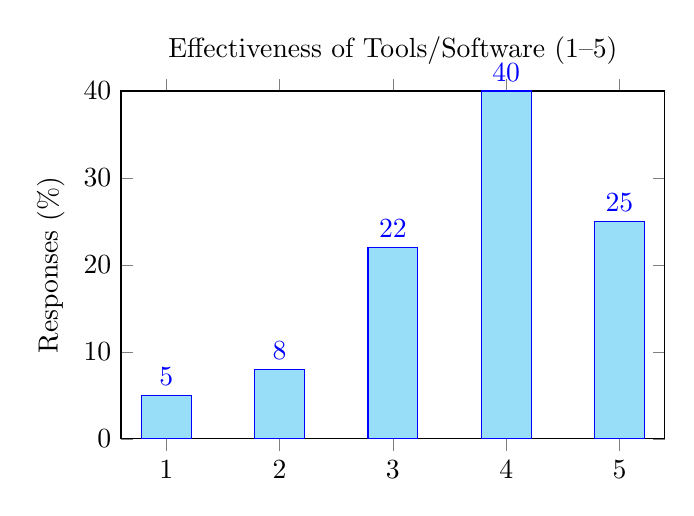
\begin{tikzpicture}
        \begin{axis}[
            ybar,
            bar width=18pt,
            width=0.7\textwidth,
            height=6cm,
            ymin=0, ymax=40,
            ylabel={Responses (\%)},
            symbolic x coords={1,2,3,4,5},
            xtick=data,
            nodes near coords,
            nodes near coords align={vertical},
            title={Effectiveness of Tools/Software (1--5)}
        ]
        \addplot+[fill=cyan!40] coordinates {(1,5) (2,8) (3,22) (4,40) (5,25)};
        \end{axis}
    \end{tikzpicture}
    \caption{How would you rate the effectiveness of the tools/software provided?}
    \label{fig:tools_effectiveness}
\end{figure}

\subsubsection*{14. Which device do you most often use to access Alpha Net's services? (Desktop/Laptop, Smartphone, Tablet)}

The majority of users access services via desktop or laptop, but mobile usage is significant and growing, highlighting the need for mobile-friendly interfaces.

\begin{figure}[H]
    \centering
    \begin{tikzpicture}
        \pie[text=legend, radius=2, color={blue!40,orange!60,green!60}]{60/Desktop-Laptop, 35/Smartphone, 5/Tablet}
    \end{tikzpicture}
    \caption{Device most often used to access Alpha Net's services}
    \label{fig:device_usage}
\end{figure}

\subsubsection*{15. How do you rate the security of Alpha Net's services? (Excellent, Good, Average, Poor)}

Most respondents rate security as good or excellent, but a small group sees room for improvement.

\begin{figure}[H]
    \centering
    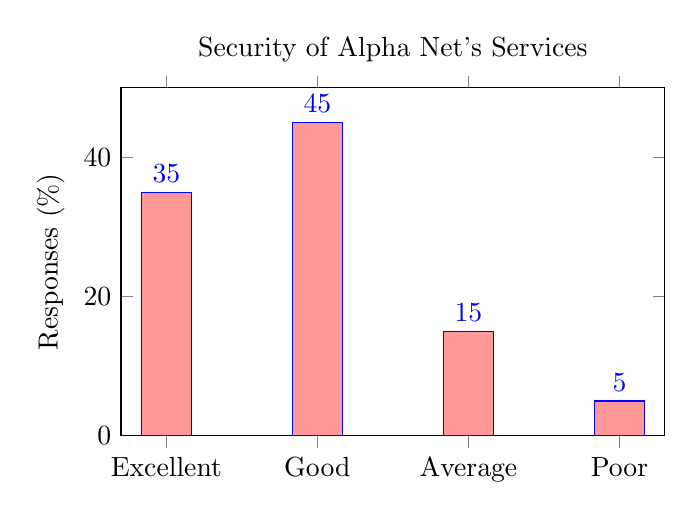
\begin{tikzpicture}
        \begin{axis}[
            ybar,
            bar width=18pt,
            width=0.7\textwidth,
            height=6cm,
            ymin=0, ymax=50,
            ylabel={Responses (\%)},
            symbolic x coords={Excellent, Good, Average, Poor},
            xtick=data,
            nodes near coords,
            nodes near coords align={vertical},
            title={Security of Alpha Net's Services}
        ]
        \addplot+[fill=red!40] coordinates {(Excellent,35) (Good,45) (Average,15) (Poor,5)};
        \end{axis}
    \end{tikzpicture}
    \caption{How do you rate the security of Alpha Net's services?}
    \label{fig:security_rating}
\end{figure}

\subsubsection*{16. What is your preferred method for receiving updates? (Email, SMS, Website Notification, Phone Call)}

Email is the most preferred method for receiving updates, followed by website notifications. SMS and phone calls are less popular.

\begin{figure}[H]
    \centering
    \begin{tikzpicture}
        \pie[text=legend, radius=2, color={blue!40,orange!60,green!60,red!40}]{50/Email, 30/Website Notification, 15/SMS, 5/Phone Call}
    \end{tikzpicture}
    \caption{Preferred method for receiving updates}
    \label{fig:update_method}
\end{figure}

\subsubsection*{17. How would you rate your work-life balance? (1--5)}

Most employees report a good work-life balance, though a minority feel it could be improved.

\begin{figure}[H]
    \centering
    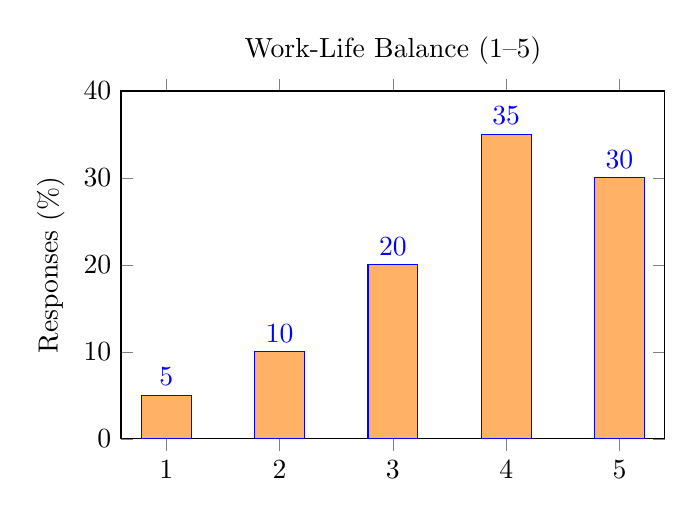
\begin{tikzpicture}
        \begin{axis}[
            ybar,
            bar width=18pt,
            width=0.7\textwidth,
            height=6cm,
            ymin=0, ymax=40,
            ylabel={Responses (\%)},
            symbolic x coords={1,2,3,4,5},
            xtick=data,
            nodes near coords,
            nodes near coords align={vertical},
            title={Work-Life Balance (1--5)}
        ]
        \addplot+[fill=orange!60] coordinates {(1,5) (2,10) (3,20) (4,35) (5,30)};
        \end{axis}
    \end{tikzpicture}
    \caption{How would you rate your work-life balance?}
    \label{fig:worklife_balance}
\end{figure}

\subsubsection*{18. How likely are you to recommend Alpha Net to others? (Very Likely, Likely, Neutral, Unlikely, Very Unlikely)}

The majority of respondents are likely or very likely to recommend Alpha Net, reflecting strong overall satisfaction.

\begin{figure}[H]
    \centering
    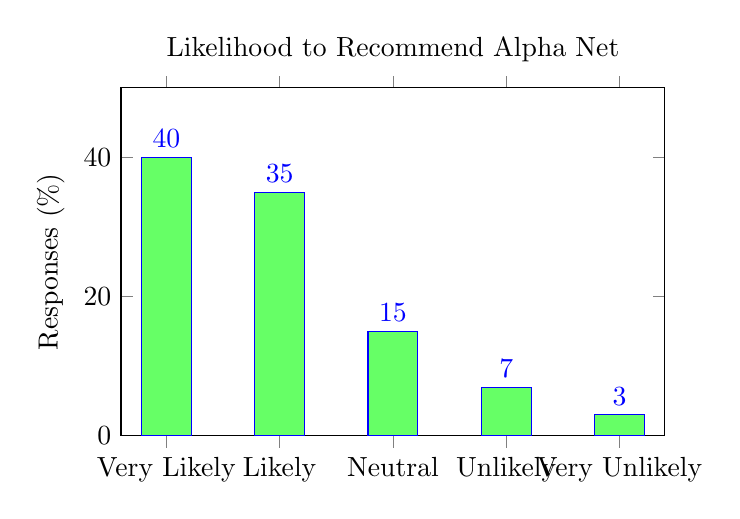
\begin{tikzpicture}
        \begin{axis}[
            ybar,
            bar width=18pt,
            width=0.7\textwidth,
            height=6cm,
            ymin=0, ymax=50,
            ylabel={Responses (\%)},
            symbolic x coords={Very Likely, Likely, Neutral, Unlikely, Very Unlikely},
            xtick=data,
            nodes near coords,
            nodes near coords align={vertical},
            title={Likelihood to Recommend Alpha Net}
        ]
        \addplot+[fill=green!60] coordinates {(Very Likely,40) (Likely,35) (Neutral,15) (Unlikely,7) (Very Unlikely,3)};
        \end{axis}
    \end{tikzpicture}
    \caption{How likely are you to recommend Alpha Net to others?}
    \label{fig:recommend_likelihood}
\end{figure}

Most employees would recommend Alpha Net, reflecting overall satisfaction, though a small minority would not.

\subsubsection*{Analysis Summary}

The above visualizations and detailed breakdowns provide a comprehensive overview of the new questions. Most employees are satisfied with the work environment and would recommend Alpha Net as a workplace. In-office work is preferred, and health benefits are most valued. Some areas, such as workload distribution and management valuing suggestions, show room for improvement.

\subsection{DFDs of Existing System}
Data Flow Diagrams (DFDs) are used to represent the flow of data through a system. The following DFDs illustrate two key processes within Alpha Net's existing operations: the customer hosting service buying process and the customer support process.

\subsubsection*{DFD for Customer Hosting Service Buying Process}
This DFD (Figure \ref{fig:dfd_buying}) illustrates the sequence of data flows when a customer purchases a hosting service from Alpha Net. The process begins with the customer browsing services and ends with the activation of the purchased service. The process is structured as follows:

\begin{itemize}
    \item \textbf{Initial Customer Interaction:}
    \begin{itemize}
        \item Customers access Alpha Net's website through desktop or mobile interfaces
        \item They browse available hosting packages and service descriptions
        \item Initial customer data (IP address, browsing patterns) is captured for analytics
        \item Product specifications and pricing information flow to the customer
    \end{itemize}

    \item \textbf{Service Selection Process:}
    \begin{itemize}
        \item Customer selects desired hosting package based on requirements
        \item Selection parameters include server specifications, bandwidth requirements, and storage needs
        \item System performs real-time availability check of requested resources
        \item Customer receives immediate feedback on service availability
    \end{itemize}

    \item \textbf{Customer Information Processing:}
    \begin{itemize}
        \item System collects comprehensive customer data including:
        \begin{itemize}
            \item Personal/business contact information
            \item Technical requirements and preferences
            \item Service duration (monthly, annual, or custom periods)
            \item Special configuration requests if applicable
        \end{itemize}
        \item Data validation occurs to ensure completeness and accuracy
        \item Customer profile is created or updated in the central database
    \end{itemize}

    \item \textbf{Payment Processing Workflow:}
    \begin{itemize}
        \item Multiple payment options are presented to the customer:
        \begin{itemize}
            \item Mobile banking (bKash, Nagad, Rocket)
            \item Traditional banking (direct deposit, bank transfer)
            \item International payment gateways (PayPal, Stripe)
            \item Credit/debit card processing
        \end{itemize}
        \item System initiates secure payment transaction
        \item Payment verification occurs in real-time
        \item Transaction data is recorded in financial database
        \item Receipt generation and delivery occurs automatically
    \end{itemize}

    \item \textbf{Service Provisioning System:}
    \begin{itemize}
        \item Upon payment confirmation, automated resource allocation begins
        \item Server resources are allocated based on package specifications
        \item Customer credentials are generated (usernames, passwords, access keys)
        \item DNS configurations are established if domain services were purchased
        \item Security protocols and firewalls are configured according to service level
    \end{itemize}

    \item \textbf{Notification and Delivery System:}
    \begin{itemize}
        \item Automated email notifications are sent containing:
        \begin{itemize}
            \item Account activation confirmation
            \item Login credentials and security information
            \item Server access details and control panel links
            \item Getting started documentation and tutorials
        \end{itemize}
        \item SMS notifications for critical information (optional)
        \item Customer database is updated with service status and specifications
    \end{itemize}

    \item \textbf{Premium Client Handling:}
    \begin{itemize}
        \item Corporate or premium clients enter a specialized workflow
        \item Technical consultants are assigned for personalized setup
        \item Custom configuration requests are implemented manually
        \item Additional security measures and service level agreements are established
        \item Direct communication channels are established with dedicated support
    \end{itemize}

    \item \textbf{Data Storage and Management:}
    \begin{itemize}
        \item Customer information is stored in centralized customer database
        \item Service specifications are recorded in service management system
        \item Transaction details are maintained in financial records
        \item Technical configurations are documented in infrastructure database
        \item All systems maintain data integrity through regular synchronization
    \end{itemize}

    \item \textbf{Post-Purchase Integration:}
    \begin{itemize}
        \item New account data flows to the billing system for recurring charges
        \item Technical support system receives new client information
        \item Resource monitoring systems begin tracking the new deployment
        \item Analytics systems incorporate new customer data for business intelligence
    \end{itemize}
\end{itemize}

The diagram highlights Alpha Net's partially automated service procurement system, with 
significant automation in standard workflows but manual intervention still required for 
premium clients and non-standard configurations. This hybrid approach balances efficiency 
with personalized service delivery.


\begin{figure}[H]
    \centering
    \begin{tikzpicture}[
        node distance=2.5cm and 2.5cm,
        every node/.style={font=\footnotesize\sffamily},
        process/.style={circle, draw, fill=blue!10, minimum size=2cm, text width=2.2cm, align=center},
        entity/.style={rectangle, draw, fill=green!20, minimum size=1.5cm, text width=2.2cm, align=center},
        datastore/.style={draw, rectangle, fill=orange!20, minimum height=1.2cm, text width=2.5cm, align=center, inner sep=4pt},
        arrow/.style={->, >=stealth, thick}
    ]
        % Entities
        \node[entity] (customer) {Customer};
        \node[entity, right=12cm of customer] (payment_gw) {Payment Gateway};
        \node[entity, below=14cm of payment_gw] (admin) {Admin/System};

        % Processes
        \node[process, below=3cm of customer] (browse) {1.0\\Select Service};
        \node[process, right=2cm of browse] (register) {2.0\\Create Account};
        \node[process, right=of register] (checkout) {3.0\\Checkout};
        \node[process, right=2cm of checkout] (payment) {4.0\\Process Payment};
        \node[process, below=4cm of checkout] (provision) {5.0\\Provision Service};
        \node[process, below=4cm of browse] (notify) {6.0\\Notify Customer};

        % Data Stores
        \node[datastore, below=2cm of browse] (services) {D1: Service Catalog};
        \node[datastore, below=2cm of register] (cart) {D4: Shopping Cart};
        \node[datastore, below=2cm of payment] (orders) {D3: Orders};
        \node[datastore, below=4cm of provision] (accounts) {D2: Customer Accounts};

        % Data Flows
        % Customer interaction
        \draw[arrow] (customer) -- node[midway, right] {Browse} (browse);
        \draw[arrow] (browse) -- node[midway, above, sloped] {Service List} (customer);
        \draw[arrow] (browse) -- node[midway, right] {Read} (services);
        \draw[arrow] (browse) -- node[midway, above, sloped] {Add to Cart} (cart);
        
        \draw[arrow] (customer) to[bend left=20] node[midway, above, sloped] {Registration Info} (register);
        \draw[arrow] (register) -- node[midway, above, sloped] {Create/Update} (accounts);
        \draw[arrow] (register) -- node[midway, above] {Account Details} (checkout);
        
        \draw[arrow] (cart) -- node[midway, above, sloped] {Cart Items} (checkout);
        \draw[arrow] (checkout) -- node[midway, above, sloped] {Create Order} (orders);
        \draw[arrow] (checkout) -- node[midway, above] {Payment Details} (payment);
        
        \draw[arrow] (payment) -- node[midway, right] {Payment Request} (payment_gw);
        \draw[arrow] (payment_gw) -- node[midway, left] {Payment Status} (payment);
        \draw[arrow] (payment) -- node[midway, right] {Update Status} (orders);
        \draw[arrow] (payment) -- (provision) node[near end, below, sloped] {Activation Trigger};       
        \draw[arrow] (orders) -- node[midway, below, sloped] {Paid Order Info} (provision);
        \draw[arrow] (accounts) -- node[midway, right] {Customer Info} (provision);
        \draw[arrow] (provision) -- node[midway, below, sloped] {Update Service} (accounts);
        \draw[arrow] (provision) -- node[midway, above] {Provisioning Details} (notify);
        \draw[arrow] (provision) -- node[midway, right] {Provisioning Log} (admin);
        
        \draw[arrow] (notify) to[bend right=34] node[near start, below, sloped] {Welcome Email} (customer);
        \draw[arrow] (accounts) -- node[midway, left] {Account Info} (notify);
        
    \end{tikzpicture}
    \caption{Detailed DFD for Customer Hosting Service Buying Process}
    \label{fig:dfd_buying}
\end{figure}

\subsubsection{DFD for Customer Support Process}
This DFD (Figure \ref{fig:dfd_support}) outlines the data flow for handling customer support requests. It shows how a ticket is created, processed by the support team, escalated if necessary, and finally resolved.
This DFD (Figure \ref{fig:dfd_support}) illustrates the comprehensive flow of data through Alpha Net's customer support process. The diagram captures the entire lifecycle of a support request from initial submission to final resolution. The process is structured as follows:

\begin{itemize}
    \item \textbf{Initial Request Submission:}
    \begin{itemize}
        \item Customers submit support requests through multiple channels (web portal, email, phone, chat)
        \item Request contains issue description, account information, and priority level
        \item System acknowledges receipt of the request automatically
        \item Initial metadata is captured including timestamp and submission method
    \end{itemize}

    \item \textbf{Ticket Logging and Categorization:}
    \begin{itemize}
        \item Support system creates a formal ticket with unique identifier
        \item Request is analyzed and categorized by issue type (technical, billing, account)
        \item System assigns priority level based on service impact and customer tier
        \item Ticket is routed to appropriate support queue based on categorization
        \item Customer receives notification with ticket details and tracking information
    \end{itemize}

    \item \textbf{First-Line Support Processing:}
    \begin{itemize}
        \item Support agent reviews ticket details and customer history
        \item Knowledge base is queried for relevant solutions and troubleshooting steps
        \item Agent communicates with customer to gather additional information if needed
        \item Standard solutions are applied for common or known issues
        \item Ticket status and interaction details are continuously updated
    \end{itemize}

    \item \textbf{Issue Escalation Workflow:}
    \begin{itemize}
        \item Complex issues requiring specialized knowledge are escalated
        \item Escalation includes complete issue history and previous troubleshooting steps
        \item Technical team receives notification with detailed problem description
        \item Specialized agents or engineers analyze complex problems
        \item Inter-departmental coordination occurs for multi-faceted issues
        \item Status updates flow back to the customer throughout escalation
    \end{itemize}

    \item \textbf{Resolution and Notification Process:}
    \begin{itemize}
        \item Once resolved, comprehensive solution documentation is prepared
        \item Resolution details are recorded in the ticketing system
        \item Customer is notified of the resolution through preferred communication channel
        \item Feedback request is automatically generated to assess satisfaction
        \item Knowledge base is updated with new solutions for future reference
        \item Ticket data flows to analytics systems for performance measurement
    \end{itemize}

    \item \textbf{Data Management and Integration:}
    \begin{itemize}
        \item All support interactions are stored in centralized ticket repository
        \item Knowledge base is continuously updated with new solutions and procedures
        \item Customer account records are enriched with support history
        \item Support metrics are calculated for quality assurance and reporting
        \item Historical data is archived according to retention policies
    \end{itemize}
\end{itemize}

The diagram reveals Alpha Net's semi-automated support workflow with significant human intervention still required for complex issue resolution. The process effectively balances standardized procedures with personalized support, though opportunities exist for enhanced automation and knowledge management.

\begin{figure}[H]
    \centering
    \begin{tikzpicture}[
        node distance=3cm and 4cm, % increased distances
        every node/.style={font=\footnotesize\sffamily},
        process/.style={circle, draw, fill=blue!10, minimum size=2cm, text width=2.2cm, align=center},
        entity/.style={rectangle, draw, fill=green!20, minimum size=1.5cm, text width=2.2cm, align=center},
        datastore/.style={draw, rectangle, fill=orange!20, minimum height=1.2cm, text width=2.5cm, align=center, inner sep=4pt},
        arrow/.style={->, >=stealth, thick}
    ]
        % Entities
        \node[entity] (customer) {Customer};
        \node[entity, right=10cm of customer] (tech_team) {Technical Team};

        % Processes
        \node[process, below=3cm of customer] (submit) {1.0\\Submit Request};
        \node[process, right=4.5cm of submit] (log) {2.0\\Log \& Categorize Ticket};
        \node[process, right=4.5cm of log] (support) {3.0\\Provide Support};
        \node[process, below=3cm of support] (escalate) {4.0\\Escalate Issue};
        \node[process, left=4.5cm of escalate] (resolve) {5.0\\Resolve \& Notify};

        % Data Stores
        \node[datastore, below=8cm of log] (tickets) {D1: Support Tickets};
        \node[datastore, below=3cm of submit] (kb) {D2: Knowledge Base};

        % Data Flows
        \draw[arrow] (customer) -- node[midway, above] {Support Request} (submit);
        \draw[arrow] (submit) -- node[midway, above] {New Request} (log);
        \draw[arrow] (log) to[bend right=30] node[midway, left] {Create/Update} (tickets);
        \draw[arrow] (log) -- node[midway, above] {Categorized Ticket} (support);
        
        \draw[arrow] (support) -- node[near start, above, sloped] {Search Solution} (kb);
        \draw[arrow] (kb) -- node[near end, below, sloped] {Solution Article} (support);
        \draw[arrow] (support) -- node[midway, right] {Update Ticket} (tickets);
        \draw[arrow] (support) -- node[midway, above, sloped] {Escalation Request} (escalate);
        \draw[arrow] (support) -- (resolve);
        
        \draw[arrow] (escalate) -- node[near start, below, sloped] {Issue Details} (tech_team);
        \draw[arrow] (tech_team) -- node[near start, below, sloped] {Technical Solution} (escalate);
        \draw[arrow] (escalate) -- node[midway, below, sloped] {Resolution Details} (resolve);
        
        \draw[arrow] (resolve) -- node[near end, above, sloped] {Final Response} (customer);
        \draw[arrow] (resolve) -- node[midway, right] {Update Resolution} (tickets);
    \end{tikzpicture}
    \caption{DFD for Customer Support Process}
    \label{fig:dfd_support}
\end{figure}

\subsubsection{DFDs of Problems}

This section presents the Data Flow Diagrams (DFDs) for the problems identified in Chapter 2. These diagrams provide a visual representation of the data flow and processes involved in addressing the key challenges.

\paragraph{Problem 1: Limited Technical Awareness Among SME Clients}
This problem highlights the challenges faced by SME clients in understanding and utilizing the technical services offered by Alpha Net. Many clients lack the necessary technical knowledge to make informed decisions about hosting services, leading to confusion and inefficiencies in service utilization. The DFD below illustrates the data flow and processes involved in addressing this issue, including client education, simplified service selection, and enhanced support mechanisms.

\begin{figure}[H]
    \centering
    \resizebox{0.95\textwidth}{!}{%
    \begin{tikzpicture}[
        node distance=2.5cm and 3cm,
        every node/.style={font=\footnotesize\sffamily},
        process/.style={circle, draw, fill=blue!10, minimum size=2cm, text width=2.2cm, align=center},
        entity/.style={rectangle, draw, fill=green!20, minimum size=1.2cm, text width=2cm, align=center},
        datastore/.style={draw, rectangle, fill=orange!20, minimum height=1cm, text width=2.2cm, align=center, inner sep=3pt},
        arrow/.style={->, >=stealth, thick}
    ]
        % External Entities
        \node[entity] (sme_client) {SME Client};
        \node[entity, right=8cm of sme_client] (tech_advisor) {Tech Advisor / Consultant};
        \node[entity, below=6cm of tech_advisor] (feedback_reports) {Feedback \& Misalignment Reports};

        % Processes
        \node[process, below=2.5cm of sme_client] (analyze1) {1.0\\Analyze Technical Awareness};
        \node[process, below=2.5cm of analyze1] (analyze2) {2.0\\Analyze Technical Awareness};
        \node[process, below=2.5cm of analyze2] (track_feedback) {5.0\\Track Feedback \& Satisfaction};

        % Data Stores
        \node[datastore, right=3cm of analyze2] (service_catalog) {D2\\Service Catalog};

        % Data Flows
        % SME Client to Process 1.0
        \draw[arrow] (sme_client) -- node[midway, left, font=\scriptsize] {SME Preferences} (analyze1);
        
        % Process 1.0 to Tech Advisor
        \draw[arrow] (analyze1) -- node[midway, above, font=\scriptsize] {Analyst Input} (tech_advisor);
        
        % Process 1.0 to Process 2.0
        \draw[arrow] (analyze1) -- node[midway, left, font=\scriptsize] {Awareness Level + Needs} (analyze2);
        
        % SME Client to Process 2.0
        \draw[arrow] (sme_client) to[bend right=25] node[near start, left, font=\scriptsize] {SME Client Needs} (analyze2);
        
        % Process 2.0 to Service Catalog
        \draw[arrow] (analyze2) -- node[midway, above, font=\scriptsize] {Confirmed Services} (service_catalog);
        
        % Service Catalog to Process 2.0
        \draw[arrow] (service_catalog) to[bend left=15] node[near end, below, font=\scriptsize] {Configured Services} (analyze2);
        
        % Process 2.0 to Process 5.0
        \draw[arrow] (analyze2) -- node[midway, left, font=\scriptsize] {Confirmed Recommendations} (track_feedback);
        
        % Tech Advisor to Service Catalog
        \draw[arrow] (tech_advisor) to[bend left=30] node[near start, right, font=\scriptsize] {Feedback Data} (service_catalog);
        
        % Process 5.0 to Feedback Reports
        \draw[arrow] (track_feedback) -- node[midway, above, font=\scriptsize] {Track Feedback} (feedback_reports);
        
        % Feedback Reports to Process 5.0
        \draw[arrow] (feedback_reports) to[bend left=15] node[near end, below, font=\scriptsize] {Feedback \& Misalignment Reports} (track_feedback);
        
    \end{tikzpicture}%
    }
    \caption{DFD for Problem 1: Limited Technical Awareness Among SME Clients}
    \label{fig:problem1_dfd}
\end{figure}

\clearpage

\paragraph{Problem 2: Fragmented Internal Communication Between Cross-Functional Teams}
This problem focuses on the inefficiencies caused by a lack of streamlined communication between different departments within Alpha Net. Fragmented communication leads to delays in issue resolution, duplication of efforts, and reduced overall productivity. The DFD below illustrates the data flow and processes involved in addressing this issue, including the implementation of centralized communication tools, regular inter-departmental meetings, and improved documentation practices.

\begin{figure}[H]
    \centering
    \resizebox{0.95\textwidth}{!}{%
    \begin{tikzpicture}[
        node distance=4cm and 5cm,
        every node/.style={font=\footnotesize\sffamily},
        process/.style={circle, draw, fill=blue!10, minimum size=2.5cm, text width=2.8cm, align=center},
        entity/.style={rectangle, draw, fill=green!20, minimum size=1.5cm, text width=2.8cm, align=center},
        datastore/.style={draw, rectangle, fill=orange!20, minimum height=1.2cm, text width=3cm, align=center, inner sep=4pt},
        arrow/.style={->, >=stealth, thick}
    ]
        % External Entities
        \node[entity] (customer) {Customer};
        \node[entity, below=8cm of customer] (handle) {Handle};
        \node[entity, right=12cm of customer] (management) {Management};
        
        % Processes
        \node[process, below=3cm of customer, right=3cm] (receive_route) {01\\Receive and Route Internal Requests};
        \node[process, below=4cm of receive_route, left=2cm] (handle_inquiries) {02\\Handle Customer Inquiries};
        \node[process, below=4cm of receive_route, right=2cm] (coordinate_updates) {03\\Coordinate Cross-Functional Updates};
        
        % Data Stores
        \node[datastore, right=4cm of receive_route] (request_log) {D3\\Internal Request Log};
        \node[datastore, below=4cm of management] (performance_reports) {D4\\Performance Reports};
        
        % Data Flows
        % Customer to Process 01
        \draw[arrow] (customer) -- node[midway, above, sloped, font=\scriptsize] {Customer Request} (receive_route);
        
        % Customer to Process 02
        \draw[arrow] (customer) to[bend right=20] node[near start, left, font=\scriptsize] {Customer Inquiry} (handle_inquiries);
        
        % Process 01 to Request Log
        \draw[arrow] (receive_route) -- node[midway, above, font=\scriptsize] {Log Request} (request_log);
        
        % Request Log to Management
        \draw[arrow] (request_log) to[bend left=15] node[near end, above, font=\scriptsize] {Request Data} (management);
        
        % Process 01 to Process 03
        \draw[arrow] (receive_route) -- node[midway, right, font=\scriptsize] {Internal Requests} (coordinate_updates);
        
        % Process 02 to Process 03
        \draw[arrow] (handle_inquiries) -- node[midway, above, font=\scriptsize] {Customer Data} (coordinate_updates);
        
        % Process 03 to Handle
        \draw[arrow] (coordinate_updates) to[bend right=30] node[near end, below, font=\scriptsize] {Coordinated Response} (handle);
        
        % Management to Performance Reports
        \draw[arrow] (management) -- node[midway, right, font=\scriptsize] {Performance Data} (performance_reports);
        
        % Performance Reports to Management (feedback loop)
        \draw[arrow] (performance_reports) to[bend left=20] node[near start, below, font=\scriptsize] {Reports} (management);
        
    \end{tikzpicture}%
    }
    \caption{DFD for Problem 2: Fragmented Internal Communication Between Cross-Functional Teams}
    \label{fig:problem2_dfd}
\end{figure}
\clearpage

\paragraph{Problem 3: Absence of Intelligent Automation in Customer Support and Infrastructure Monitoring}
The lack of intelligent automation in customer support and infrastructure monitoring leads to inefficiencies and increased workload for the support team. Manual processes dominate issue resolution, resulting in slower response times and higher operational costs. Additionally, the absence of proactive monitoring tools increases the risk of service disruptions and delays in identifying potential issues. The DFD below illustrates the data flow and processes involved in addressing this problem, including the integration of AI-powered chatbots, automated ticket categorization, and real-time infrastructure monitoring systems.

\begin{figure}[H]
    \centering
    \resizebox{0.9\textwidth}{!}{%
    \begin{tikzpicture}[
        node distance=3cm and 3.5cm,
        every node/.style={font=\footnotesize\sffamily},
        process/.style={circle, draw, fill=blue!10, minimum size=2.5cm, text width=2.8cm, align=center},
        entity/.style={rectangle, draw, fill=green!20, minimum height=1cm, text width=2.8cm, align=center},
        datastore/.style={draw, cylinder, shape border rotate=90, 
            aspect=0.35, fill=orange!20, minimum height=1.8cm, minimum width=1.2cm, text width=3.2cm, align=center},
        arrow/.style={->, >=stealth, thick}
    ]

        % External Entities
        \node[entity] (customer) {Customer};
        \node[entity, right=9cm of customer] (servers_systems) {Servers / Systems};
        \node[entity, below=6cm of servers_systems] (knowledge_base) {Knowledge Base};
        
        % Processes
        \node[process, below=2.8cm of customer, right=2.5cm] (receive_support) {Receive Support Request};
        \node[process, below=4cm of receive_support] (manual_handling) {Manual Ticket Handling};
        
        % Data Store (cylinder style for clarity)
        \node[datastore, right=4.5cm of manual_handling] (system_logs) {System Logs / Monitoring Data};
        
        % Data Flows
        % Customer to Receive Support Request
        \draw[arrow] (customer) -- node[midway, above, sloped, font=\scriptsize] {Ticket} (receive_support);
        
        % Receive Support Request to Servers/Systems
        \draw[arrow] (receive_support) -- node[midway, above, font=\scriptsize] {Logs} (servers_systems);
        \draw[arrow] (receive_support) to[bend left=10] node[near start, above, font=\scriptsize] {Metrics} (servers_systems);
        
        % Receive Support Request to Manual Ticket Handling
        \draw[arrow] (receive_support) -- node[midway, left, font=\scriptsize] {Response} (manual_handling);
        
        % Servers/Systems to System Logs
        \draw[arrow] (servers_systems) -- node[midway, right, font=\scriptsize] {Monitoring Data} (system_logs);
        
        % System Logs to Manual Ticket Handling
        \draw[arrow] (system_logs) -- node[midway, above, font=\scriptsize] {Infra Monitoring} (manual_handling);
        
        % Manual Ticket Handling to Knowledge Base
        \draw[arrow] (manual_handling) -- node[midway, above, sloped, font=\scriptsize] {Knowledge} (knowledge_base);
        
        % Knowledge Base to Manual Ticket Handling
        \draw[arrow] (knowledge_base) to[bend left=15] node[near end, below, font=\scriptsize] {Alerts} (manual_handling);
        
    \end{tikzpicture}%
    }
    \caption{DFD for Problem 3: Absence of Intelligent Automation in Customer Support and Infrastructure Monitoring}
    \label{fig:problem3_dfd}
\end{figure}

\clearpage

\paragraph{Problem 4: Overdependence on Upstream Infrastructure Providers Risks Service Continuity}
This problem addresses Alpha Net's vulnerability due to its heavy reliance on external infrastructure providers. Service disruptions from upstream providers can cascade to Alpha Net's clients, affecting business continuity and customer satisfaction. The lack of redundancy and failover mechanisms increases the risk of extended outages. The DFD below illustrates the data flow and processes involved in addressing this challenge, including infrastructure diversification, implementation of real-time monitoring across providers, automated failover mechanisms, and enhanced disaster recovery protocols. This approach aims to create a more resilient service architecture that can maintain continuity even when individual providers experience issues.
\begin{figure}[H]
    \centering
    \resizebox{0.9\textwidth}{!}{%
    \begin{tikzpicture}[
        node distance=2.8cm and 3.5cm,
        every node/.style={font=\footnotesize\sffamily},
        process/.style={circle, draw, fill=blue!15, minimum size=2.5cm, text width=2.8cm, align=center, font=\bfseries},
        entity/.style={rectangle, draw, fill=green!20, minimum height=1cm, text width=3cm, align=center},
        datastore/.style={cylinder, draw, shape border rotate=90, aspect=0.35, 
            fill=orange!20, minimum height=1.5cm, minimum width=1.2cm, text width=3cm, align=center},
        arrow/.style={->, >=stealth, thick}
    ]
        % External Entities
        \node[entity] (customer) {Customer};
        \node[entity, right=9cm of customer] (upstream_provider) {Upstream Infrastructure Provider};
        \node[entity, below=6cm of customer] (management) {Management};
        
        % Processes
        \node[process, below=2.5cm of customer, right=2cm] (accept_service) {01 \\ Accept Service Request};
        \node[process, below=3.2cm of accept_service, right=2.5cm] (manage_operations) {02 \\ Manage Service Operations};
        \node[process, left=3cm of manage_operations] (manage_database) {02 \\ Manage Service Database};
        \node[process, below=3cm of manage_operations] (provision_infra) {03 \\ Provision Infrastructure};
        
        % Data Stores
        \node[datastore, below=2.5cm of manage_operations] (service_data) {D2 \\ Service Data};
        \node[datastore, below=2.5cm of management] (service_metrics) {D1 \\ Service Metrics};
        
        % Data Flows
        \draw[arrow] (customer) -- node[midway, above, sloped, font=\scriptsize] {Service Request} (accept_service);
        \draw[arrow] (accept_service) -- node[midway, above, font=\scriptsize] {Infrastructure Request} (upstream_provider);
        \draw[arrow] (accept_service) -- node[midway, right, font=\scriptsize] {Service Details} (manage_operations);
        \draw[arrow] (upstream_provider) to[bend right=20] node[near start, right, font=\scriptsize] {Infrastructure Status} (manage_operations);
        
        \draw[arrow] (manage_operations) -- node[midway, right, font=\scriptsize] {Service Config} (service_data);
        \draw[arrow] (service_data) -- node[midway, above, font=\scriptsize] {Config Data} (provision_infra);
        
        \draw[arrow] (manage_database) to[bend left=15] node[near end, above, font=\scriptsize] {Database Updates} (service_data);
        \draw[arrow] (manage_database) -- node[midway, above, sloped, font=\scriptsize] {Performance Data} (service_metrics);
        
        \draw[arrow] (management) -- node[midway, above, font=\scriptsize] {Metrics Request} (service_metrics);
        \draw[arrow] (service_metrics) to[bend left=15] node[near start, below, font=\scriptsize] {Service Reports} (management);
        
        \draw[arrow] (manage_operations) -- node[midway, above, font=\scriptsize] {Operation Data} (manage_database);
        
    \end{tikzpicture}%
    }
    \caption{DFD for Problem 4: Overdependence on Upstream Infrastructure Providers Risks Service Continuity}
    \label{fig:problem4_dfd}
\end{figure}
